% ============================================================================
%  Conditional Lead-Lag Alpha -- Final Report (MFE 230GA)
%  Compile twice (for cross-references) with pdfLaTeX or LuaLaTeX, e.g.
%      pdflatex final_report.tex && pdflatex final_report.tex
%  On Overleaf: upload this folder plus the two figures and press Recompile.
%  This file holds the preamble and Sections 1-3. The appendices are in
%  appendices.tex (which pulls in appendix_chatgpt_p4.tex and _p5.tex).
%  Figures are read from ../figures/ (or figures/ or this folder).
% ============================================================================
\documentclass[11pt,letterpaper]{article}

\usepackage{iftex}
\ifPDFTeX
  \usepackage[utf8]{inputenc}
  \usepackage[T1]{fontenc}
  \usepackage{lmodern}
\else
  \usepackage{fontspec}   % LuaLaTeX / XeLaTeX: Latin Modern is the default font
\fi
\usepackage{newunicodechar}
\usepackage[margin=1in,headheight=14pt]{geometry}
\usepackage{microtype}
\usepackage{amsmath,amssymb}
\usepackage{graphicx}
\usepackage{float}
\usepackage{comment}
\usepackage[breakable]{tcolorbox}
\usepackage{booktabs,longtable,array,tabularx,calc}
\usepackage{caption}
\usepackage{enumitem}
\usepackage{titlesec}
\usepackage{fancyhdr}
\usepackage{fvextra}
\usepackage{xurl}
\usepackage[hidelinks]{hyperref}

\graphicspath{{../figures/}{figures/}{./}}

% ----------------------------------------------------------------------------
%  TITLE BLOCK -- edit these four lines
% ----------------------------------------------------------------------------
\newcommand{\reporttitle}{Conditional Lead-Lag Alpha}
\newcommand{\reportcourse}{MFE 230GA: Equity Markets --- Final Report}
\newcommand{\reportdate}{October 2026}
\newcommand{\reportauthors}{%
  Elias Roubache \and      % Part 1: data and universe
  Connor O'Rourke \and     % Part 2: shock identification
  Reza Zamani \and         % Part 3: signal and validation
  Thomas Claudel \and      % Part 4: portfolio and risk
  Paraj Goyal}             % Part 5: robustness and final report

% ----------------------------------------------------------------------------
%  RUNNING HEADER AND FOOTER
% ----------------------------------------------------------------------------
\pagestyle{fancy}
\fancyhf{}
\fancyhead[L]{\small\reporttitle}
\fancyhead[R]{\small MFE 230G Final Project}
\fancyfoot[C]{\small\thepage}
\renewcommand{\headrulewidth}{0.4pt}

\title{\textbf{\reporttitle}}
\author{\reportauthors}
\date{\reportcourse\\[0.2em]\reportdate}
% ----------------------------------------------------------------------------

% -- layout ------------------------------------------------------------------
\setlength{\parindent}{0pt}
\setlength{\parskip}{0.55em}
\setlength{\emergencystretch}{3em}
\setlist{itemsep=0.15em,topsep=0.2em,leftmargin=1.4em}
\captionsetup{font=small,labelfont=bf,skip=4pt}
\titlespacing*{\section}{0pt}{1.1em}{0.4em}
\titlespacing*{\subsection}{0pt}{0.8em}{0.25em}
\titleformat{\paragraph}{\normalfont\normalsize\bfseries}{}{0pt}{}
\titlespacing*{\paragraph}{0pt}{0.7em}{0.15em}
\titleformat{\subparagraph}{\normalfont\normalsize\itshape}{}{0pt}{}
\titlespacing*{\subparagraph}{0pt}{0.6em}{0.1em}
\setcounter{secnumdepth}{2}
\newcolumntype{Y}{>{\raggedright\arraybackslash}X}
\newcommand{\file}[1]{\texttt{\small #1}}

% -- needed by the converted ChatGPT transcripts -----------------------------
\providecommand{\tightlist}{\setlength{\itemsep}{0pt}\setlength{\parskip}{0pt}}
\RecustomVerbatimEnvironment{verbatim}{Verbatim}{breaklines,breakanywhere,fontsize=\footnotesize}
\newunicodechar{→}{\ensuremath{\rightarrow}}
\newunicodechar{Σ}{\ensuremath{\Sigma}}
\newunicodechar{−}{\ensuremath{-}}
\newunicodechar{⁻}{\ensuremath{{}^{-}}}
\newunicodechar{⁺}{\ensuremath{{}^{+}}}
\newunicodechar{¹}{\ensuremath{{}^{1}}}
\newunicodechar{ᵀ}{\ensuremath{{}^{\top}}}
\newunicodechar{×}{\ensuremath{\times}}
\newunicodechar{√}{\ensuremath{\surd}}
\newunicodechar{÷}{\ensuremath{\div}}

\begin{document}
\maketitle
\thispagestyle{fancy}

% ============================================================================
\section{Executive Summary}
% ============================================================================

\textbf{Do not implement.} We proposed a conditional lead-lag strategy on US
stocks: each day, split the return of every industry's largest stock (the
``leader'') into a part shared with the market and industry and a part specific
to the leader, then buy followers after common moves and sell them after
leader-specific moves. On CRSP daily data for 1996--2024, leaders do predict
their followers' next-day returns (coefficient 0.0093, $t = 5.03$), but the
result does not support the strategy. The effect is continuation rather than
reversal, it is confined to 1996--2006, and followers do not revert on the
leader-specific shock, so the conditional signal is weaker than its own common
leg. Built as a dollar-, beta- and own-lag-neutral book traded open to close,
the conditional signal earns $-0.46\%$ a year ($t = -1.08$). The best
leader-based book earns $0.85\%$ a year before costs and breaks even at a
one-way cost of 0.17~bp, against a median quoted half-spread of 2.58~bp. Paying
that half-spread turns every book's return into a loss of 10\% to 13\% a year.

% ============================================================================
\section{What Did We Try?}
% ============================================================================

\subsection{Ideas}

The idea starts from industry lead-lag: large firms' returns predict the later
returns of smaller firms in the same industry, usually read as slow diffusion
of information. We asked whether the direction of the follower's response
depends on why the leader moved. If the leader moves with its industry,
followers should continue in the same direction. If the move is specific to the
leader, followers that are dragged along should revert. That gave four
hypotheses (Table~\ref{tab:hyp}). The strategy that follows from H1 and H2 is
one number per follower per day: the common part of the leader's previous-day
return minus the leader-specific part.

\begin{table}[h]
\centering\small
\caption{Hypotheses and outcomes.}\label{tab:hyp}
\begin{tabularx}{\textwidth}{@{}lYll@{}}
\toprule
 & Hypothesis & Tested in & Outcome \\
\midrule
H1 & Followers continue on the common (market and industry) part of the leader's move & Parts 2--3 & Supported \\
H2 & Followers revert on the leader-specific shock & Parts 2--3 & Not supported \\
H3 & Conditioning on the source of the move beats the unconditional leader signal and plain short-term reversal & Parts 3--4 & Rejected \\
H4 & The signal stays economically meaningful after risk controls, turnover and costs & Parts 4--5 & Rejected \\
\bottomrule
\end{tabularx}
\end{table}

\subsection{Data}

All results use CRSP daily data for 1996--2024, pulled through WRDS, with no
survivorship or look-ahead bias by construction (Table~\ref{tab:data}). The
size screen removes the most stocks (56\% fail it on its own), then the price
screen (24\%). Licensed stock-level data is not in the public repository; every
table regenerates from code.

\begin{table}[h]
\centering\small
\caption{Data and universe.}\label{tab:data}
\begin{tabularx}{\textwidth}{@{}lY@{}}
\toprule
Item & Detail \\
\midrule
Sources & CRSP daily stock file, delistings and name history; Fama-French five factors and momentum (Ken French Data Library, via WRDS); Databento one-minute quotes for an intraday pilot \\
Sample & 1996--2024, 34.4 million CRSP rows, 7,173 trading sessions \\
Industries & Fama-French 49, assigned point-in-time from CRSP name history, with ``Other'' excluded (48 used) \\
Universe & Monthly, five screens: observation count, \$5 price floor, NYSE size floor, liquidity, industry not ``Other''. About 1,747 eligible stocks a month \\
Leaders, followers & Leader = largest firm in each industry using data through the previous month; all other eligible firms are followers. Monthly leader turnover is 5.4\% \\
Panel & 12.4 million follower-days \\
Survivorship & Delisting returns merged in; Shumway's substitute for 417 missing performance delistings \\
Look-ahead control & Every conditioning variable is taken at the previous close \\
\bottomrule
\end{tabularx}
\end{table}

\subsection{Implementation}

The work ran in five steps, each built on the previous one's code, with unit
tests on a synthetic panel with a planted effect.

\textbf{Baseline (Part 1).} Daily Fama-MacBeth regressions of follower returns
on the leader's lagged return, controlling for the follower's own lagged
return, with Newey-West standard errors:
\[
r_{i,t} = a_t + b_t\, r_{L(i),\,t-k} + c_t\, r_{i,\,t-k} + \varepsilon_{i,t}.
\]

\textbf{Shock decomposition (Part 2).} Each day the leader's return is
regressed, on a rolling point-in-time window, on the market and an industry
index that excludes the leader. The fitted part is the common component; the
residual is the leader-specific shock:
\[
r_{L,t} = \alpha + \beta_m\, \mathrm{MKT}_t + \beta_j\,
\mathrm{IND}^{\text{ex-leader}}_{j,t} + u_{L,t}, \qquad
\mathrm{common}_t = r_{L,t} - u_{L,t}, \quad \mathrm{shock}_t = u_{L,t}.
\]
On average the common component explains about 40\% of a leader's daily
variance.

\textbf{Signal and validation (Part 3).} The conditional signal is the lagged
common component minus the lagged shock. It is scored by daily cross-sectional
rank IC at horizons of 1, 5, 10 and 20 days and by quintile long-short
portfolios, against two baselines: the unconditional leader return and the
follower's own-return reversal.

\textbf{Portfolio and risk (Part 4).} The design was written down before any
result was computed.
\begin{itemize}
\item \textbf{Construction.} The leader signals take one value per industry,
  so the real breadth is 48 industries. Each day industries are ranked on the
  signal and the ranks are made neutral to dollar, market beta and the
  industry's own previous-day return. Each industry's weight is split equally
  across its followers, at gross exposure 1.
\item \textbf{Risk modeling.} Betas are Dimson betas over 252 sessions, shrunk
  halfway to one. Books are sized by gross exposure and realized volatility;
  there is no full factor risk model. Risk is measured by drawdown, 99\%
  historical VaR with Kupiec backtests, and three stress periods.
\item \textbf{Timing.} The headline book is formed from information at the
  previous close, bought at the open and sold at the same day's close.
  Close-to-close is reported as an upper bound.
\item \textbf{Turnover and costs.} An open-to-close book is flat overnight, so
  it trades twice its gross exposure every day. Costs are measured as the
  one-way cost at which a book's return is zero, compared with the median
  quoted half-spread of the stocks held.
\item \textbf{Decision rule.} Implement only if the conditional book has a
  significantly positive mean after Holm correction, a positive alpha after
  controlling for factors and the reversal book, and a breakeven cost above
  the median half-spread.
\end{itemize}

\textbf{Robustness (Part 5).} Net-of-cost returns at a range of one-way costs,
year-by-year and sub-period returns, and midpoint-price checks, all computed
from the Part 4 daily book returns.

\textbf{ChatGPT prompts.} We used ChatGPT three times (Table~\ref{tab:prompts}).
Full prompts, outputs and our evaluation are in Appendix~\ref{app:chatgpt}.

\begin{table}[h]
\centering\small
\caption{ChatGPT prompts, in short.}\label{tab:prompts}
\begin{tabularx}{\textwidth}{@{}l>{\raggedright\arraybackslash}p{0.27\textwidth}Y@{}}
\toprule
\# & Purpose & Prompt \\
\midrule
1 & Robustness design (Part 4) & ``List every way this backtest could show a profit that would not survive in real trading, or that is not the effect I think I am measuring,'' with a detection method and fix for each \\
2 & Portfolio construction and coding (Part 4) & Propose a dollar-, beta- and own-lag-neutral construction for a signal shared within an industry, a risk model, a sizing rule, and Python for the weights \\
3 & Cost, microstructure and out-of-sample design (Part 5) & Given the turnover and breakeven numbers, propose a cost model, rank the microstructure effects that could create or hide the return, say which out-of-sample tests still count, and state in advance what would overturn ``do not implement'' \\
\bottomrule
\end{tabularx}
\end{table}

% ============================================================================
\section{What Did We Learn?}
% ============================================================================

\subsection{The signal, and its style and risk factor exposures}

\textbf{The lead-lag effect is real, but it is not the one we proposed.}
Followers respond to the common part of the leader's move (coefficient 0.0396,
$t = 7.70$) and barely to the leader-specific part (0.0034, $t = 1.86$), and
that response has the wrong sign for H2. Subtracting a leg with no reversal
from a leg that works cuts the rank IC from 0.0049 ($t = 3.52$) for the common
leg to 0.0010 ($t = 0.93$) for the conditional signal, below both baselines, so
H3 is rejected (Table~\ref{tab:evidence}).

\begin{table}[h]
\centering\small
\caption{One-day evidence from Parts 1--3.}\label{tab:evidence}
\begin{tabular}{@{}lrr@{}}
\toprule
Test (one-day lag) & Estimate & $t$ \\
\midrule
Part 1: follower return on leader's lagged return & 0.0093 & 5.03 \\
Part 2: response to common component & 0.0396 & 7.70 \\
Part 2: response to leader-specific shock & 0.0034 & 1.86 \\
Part 3: rank IC, conditional signal & 0.0010 & 0.93 \\
Part 3: rank IC, common leg alone & 0.0049 & 3.52 \\
Part 3: rank IC, own-return reversal & 0.0166 & 10.91 \\
\bottomrule
\end{tabular}
\end{table}

\textbf{The books carry almost no standard factor exposure.} In regressions on
the Fama-French five factors, momentum and the lagged market, $R^2$ is below
2\% for every lead-lag book and no Fama-French or momentum loading is
significant. The exposures that matter are the ones the construction removes.
\begin{itemize}
\item \textbf{Market beta.} Beta neutrality alone takes the conditional signal
  from 1.9\% a year ($t = 3.0$) to $-0.3\%$ ($t = -0.6$), close to close. The
  common component contains yesterday's market move, so ranking industries on
  it is largely a bet that high-beta industries keep moving with the market.
\item \textbf{Industry momentum.} Across industries the common leg has a
  correlation of 0.63 with the followers' own previous-day return, because the
  industry index is built from those followers. With all three constraints the
  common leg falls from 6.6\% a year to 1.2\%.
\item \textbf{Short-term reversal.} The common, shock and leader-return books
  load negatively on the reversal book ($t$ between $-2.4$ and $-4.9$).
\end{itemize}

\begin{table}[h]
\centering\small
\caption{Gross-1 books, open to close, 1996--2024. Newey-West $t$-statistics with 5 lags.}\label{tab:perf}
\begin{tabular}{@{}lrrrrr@{}}
\toprule
Book & Return / yr & Volatility / yr & Sharpe & $t$ & Max drawdown \\
\midrule
Conditional signal    & $-0.46\%$ & 2.3\% & $-0.20$ & $-1.08$ & $-16.6\%$ \\
Common leg            & $0.85\%$  & 2.4\% & $0.35$  & $1.90$  & $-7.6\%$ \\
Leader return         & $0.79\%$  & 2.3\% & $0.34$  & $1.80$  & $-8.1\%$ \\
Leader-specific shock & $0.77\%$  & 2.3\% & $0.34$  & $1.78$  & $-6.5\%$ \\
Reversal benchmark    & $2.52\%$  & 3.2\% & $0.78$  & $3.70$  & $-45.7\%$ \\
\bottomrule
\end{tabular}
\end{table}

None of the four pre-registered primary tests is significant after Holm
correction (Table~\ref{tab:perf}). The shock book earns a positive return under
every set of constraints, so followers continue on the leader-specific shock
instead of reverting. Tail risk is understated by a trailing window: one-day
99\% VaR from a 250-day history is breached 96 to 115 times against about 69
expected, and the Kupiec test rejects for every book. The conditional book's
worst stress period is March 2020 ($-2.4\%$).

\subsection{Time patterns of performance}

\textbf{The effect belongs to 1996--2006, and the conditional book loses money
in every long window.} In the Part 1 regression the one-day coefficient is
0.0206 ($t = 7.97$) in 1996--2006 and 0.0025 ($t = 1.02$) in 2007--2024, while
the median relative spread fell from 3.23\% to 0.11\%
(Figure~\ref{fig:byyear}).

\begin{figure}[h]
\centering
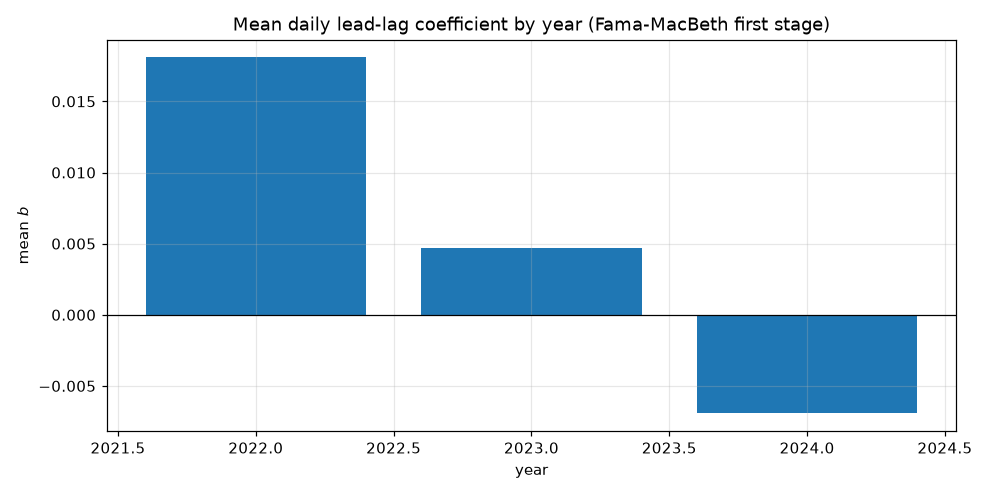
\includegraphics[width=0.62\textwidth]{p1_coefficient_by_year.png}
\caption{Part 1 lead-lag coefficient by year (annual mean of the pooled-regression coefficient on the leader's prior-day return).}\label{fig:byyear}
\end{figure}

\begin{table}[h]
\centering\footnotesize
\caption{Return per year, open to close, with the Newey-West $t$-statistic in brackets. The data end in December 2024, so the last 18 months are July 2023 to December 2024.}\label{tab:windows}
\setlength{\tabcolsep}{3.5pt}
\begin{tabular}{@{}lrrrrrr@{}}
\toprule
Book & 1996--2024 & 1996--2006 & 2007--2024 & 2010--2024 & Last 18 m & Last 12 m \\
\midrule
Conditional signal & $-0.5\%$ ($-1.1$) & $-0.4\%$ ($-0.7$) & $-0.5\%$ ($-0.9$) & $-0.7\%$ ($-1.3$) & $0.3\%$ ($0.2$) & $0.5\%$ ($0.3$) \\
Common leg         & $0.8\%$ ($1.9$) & $1.1\%$ ($1.6$) & $0.7\%$ ($1.2$) & $1.0\%$ ($1.6$) & $-2.2\%$ ($-1.3$) & $-1.3\%$ ($-0.6$) \\
Leader return      & $0.8\%$ ($1.8$) & $1.1\%$ ($1.6$) & $0.6\%$ ($1.1$) & $0.9\%$ ($1.5$) & $-1.8\%$ ($-1.2$) & $-1.5\%$ ($-0.8$) \\
Reversal benchmark & $2.5\%$ ($3.7$) & $3.0\%$ ($2.5$) & $2.2\%$ ($2.8$) & $1.9\%$ ($2.3$) & $-0.2\%$ ($-0.1$) & $-2.1\%$ ($-0.9$) \\
\bottomrule
\end{tabular}
\end{table}

The common and leader-return books lose money over the last 18 months
(Table~\ref{tab:windows}). Those windows are short: an 18-month Sharpe ratio
has a standard error of about 0.8, so they are descriptive only. Year by year,
the conditional book is positive in 12 of 29 calendar years and the common leg
in 19 of 29. Cumulative returns are in Figure~\ref{fig:cumulative}.

\subsection{Robustness and limits}

\textbf{Every check confirms ``do not implement''.} Before running them
we fixed the rule: the verdict is overturned only if a book keeps a positive
return after paying the median quoted half-spread with zero market impact, the
most favourable cost case. No book comes close.

\textbf{Transaction costs.} An open-to-close book trades twice its gross each
day, so each basis point of one-way cost removes about 5 percentage points of
annual return (Table~\ref{tab:costs}).

\begin{table}[h]
\centering\small
\caption{Net return per year, open to close, 2007--2024, by one-way cost. The last column is the median quoted half-spread of the stocks held.}\label{tab:costs}
\begin{tabular}{@{}lrrrrr@{}}
\toprule
Book & No cost & 0.1 bp & 0.5 bp & 1 bp & 2.58 bp \\
\midrule
Conditional signal    & $-0.5\%$ & $-1.0\%$ & $-3.0\%$ & $-5.5\%$ & $-13.5\%$ \\
Common leg            & $0.7\%$  & $0.2\%$  & $-1.8\%$ & $-4.3\%$ & $-12.3\%$ \\
Leader return         & $0.6\%$  & $0.1\%$  & $-1.9\%$ & $-4.4\%$ & $-12.4\%$ \\
Leader-specific shock & $0.8\%$  & $0.3\%$  & $-1.7\%$ & $-4.3\%$ & $-12.2\%$ \\
Reversal benchmark    & $2.2\%$  & $1.7\%$  & $-0.3\%$ & $-2.8\%$ & $-10.8\%$ \\
\bottomrule
\end{tabular}
\end{table}

Carrying positions overnight lowers turnover to about 1.3 a day, but the
leader-based close-to-close books still lose 7\% to 9\% a year at the median
half-spread. The cost case is weaker still in 1996--2006, where the gross
return is highest: Part 1 reports a median relative spread of 3.23\% at the
start of the sample against 0.11\% at the end, about thirty times wider.
Market impact, fees and short-borrow costs would add to these losses and are
not modelled.

\textbf{Microstructure.}
\begin{itemize}
\item \textbf{Bid-ask bounce does not drive the lead-lag effect.} On bid-ask
  midpoint returns the Part 1 coefficient is 0.0096 ($t = 5.19$) against 0.0093
  ($t = 5.03$) on closing prices. The conditional book earns $-0.78\%$ a year
  on midpoints against $-0.70\%$ on closes.
\item \textbf{Bounce does drive the reversal benchmark.} Close to close it
  earns 10.1\% a year, on midpoints 1.9\%, and in 1996--2006 it loses 1.0\% a
  year on midpoints. About 7.5 of its 10.1 points arrive overnight, which a
  trader cannot capture.
\item \textbf{Stale prices are not ruled out.} Trading from the open excludes
  the overnight catch-up of stale closes, and the leader-based books' return
  falls by 30\% to 50\% as a result. A direct test needs intraday quotes, which
  we hold only for 2018--2024, when the effect is already absent. A one-month
  pilot on 22 stocks was not significant ($t = -1.67$).
\end{itemize}

\textbf{Out-of-sample.} No holdout was reserved and the whole 1996--2024 sample
was examined during development, so every split is pseudo-out-of-sample.
Selected on 1996--2006 and evaluated on 2007--2024, the common leg earns 0.7\%
a year ($t = 1.2$) and the conditional signal $-0.5\%$ ($t = -0.9$): no
leader-based book is significant in the later period even before costs
(Table~\ref{tab:oos}). A genuine out-of-sample test needs data after December
2024 with the specification locked; we have not run one.

\begin{table}[h]
\centering\small
\caption{Pseudo-out-of-sample split, open to close: return per year (Newey-West $t$).}\label{tab:oos}
\begin{tabular}{@{}lrr@{}}
\toprule
Book & Selected on 1996--2006 & Evaluated on 2007--2024 \\
\midrule
Conditional signal & $-0.4\%$ ($t = -0.7$) & $-0.5\%$ ($t = -0.9$) \\
Common leg         & $1.1\%$ ($t = 1.6$)   & $0.7\%$ ($t = 1.2$) \\
Leader return      & $1.1\%$ ($t = 1.6$)   & $0.6\%$ ($t = 1.1$) \\
\bottomrule
\end{tabular}
\end{table}

\textbf{Limits.}
\begin{itemize}
\item Books are sized by gross exposure and realized volatility; there is no
  factor risk model, and the industry books rest on about 48 independent bets
  a day.
\item Costs use closing quoted spreads. Opening and closing auction costs are
  not measured, and Nasdaq's auctions began only in 2004, inside the period
  that produces the return.
\item The Fama-French factors exist only close to close, so the open-to-close
  attribution is approximate beyond the market factor.
\item Long and short legs separately, profit concentration by industry, and
  leave-one-industry-out tests need stock-level weights and were not run.
\end{itemize}

\subsection{ChatGPT evaluation}

\textbf{ChatGPT was a strong checklist and a weak judge of what matters for
this dataset.} We used it three times, to review the backtest design, the
portfolio construction and the robustness plan (Table~\ref{tab:gpt}).

\begin{table}[h]
\centering\small
\caption{The three ChatGPT interactions.}\label{tab:gpt}
\begin{tabularx}{\textwidth}{@{}>{\raggedright\arraybackslash}p{0.22\textwidth}YY@{}}
\toprule
Interaction & Most useful & Main flaw \\
\midrule
1. False-profit checklist & Saw unprompted that the signal is industry allocation and a market-beta bet & Moved the trade a full session late, where every book earns nothing \\
2. Construction and risk model & Agreed on the constraints; called a diagonal risk model inadequate & Weighted industries by follower count, a problem it had itself flagged \\
3. Cost and out-of-sample design & Made the spread-only test the deciding case; stricter out-of-sample labels & Ranked bounce first, though Part 1 had ruled it out \\
\bottomrule
\end{tabularx}
\end{table}

\textbf{Strengths.} It lists failure modes quickly and thoroughly, it reasons
correctly from numbers it is given, and it is candid about what a dataset
cannot identify. In the third interaction, supplying the turnover and
breakeven numbers fixed the first interaction's weakness, where it could only
say that costs ``might be decisive''.

\textbf{Limits.} It cannot rank its own list: the items that decide the result
sit among dozens that do not apply or were already handled. It follows the
prompt's framing even when the framing is the mistake, as with the execution
time. Its code needs checking: one answer lost the start of its function,
another included the same day's return in the volatility that sizes that
day's cost.

\textbf{Adaptations.} We learned to state facts and ask for the earliest
feasible choice instead of stating a choice, to supply our own numbers, to ask
for a ranking and for what does not apply, and to ask for pass/fail rules
before running a test. The pattern matches HW1 and HW2: good at saying what
could go wrong, weak at saying which of those things matters here.

% ============================================================================
%  APPENDICES (separate file)
% ============================================================================
% ============================================================================
\clearpage
\appendix
\section{Additional Tables and Figures}\label{app:tables}
% ============================================================================

\begin{figure}[h]
\centering
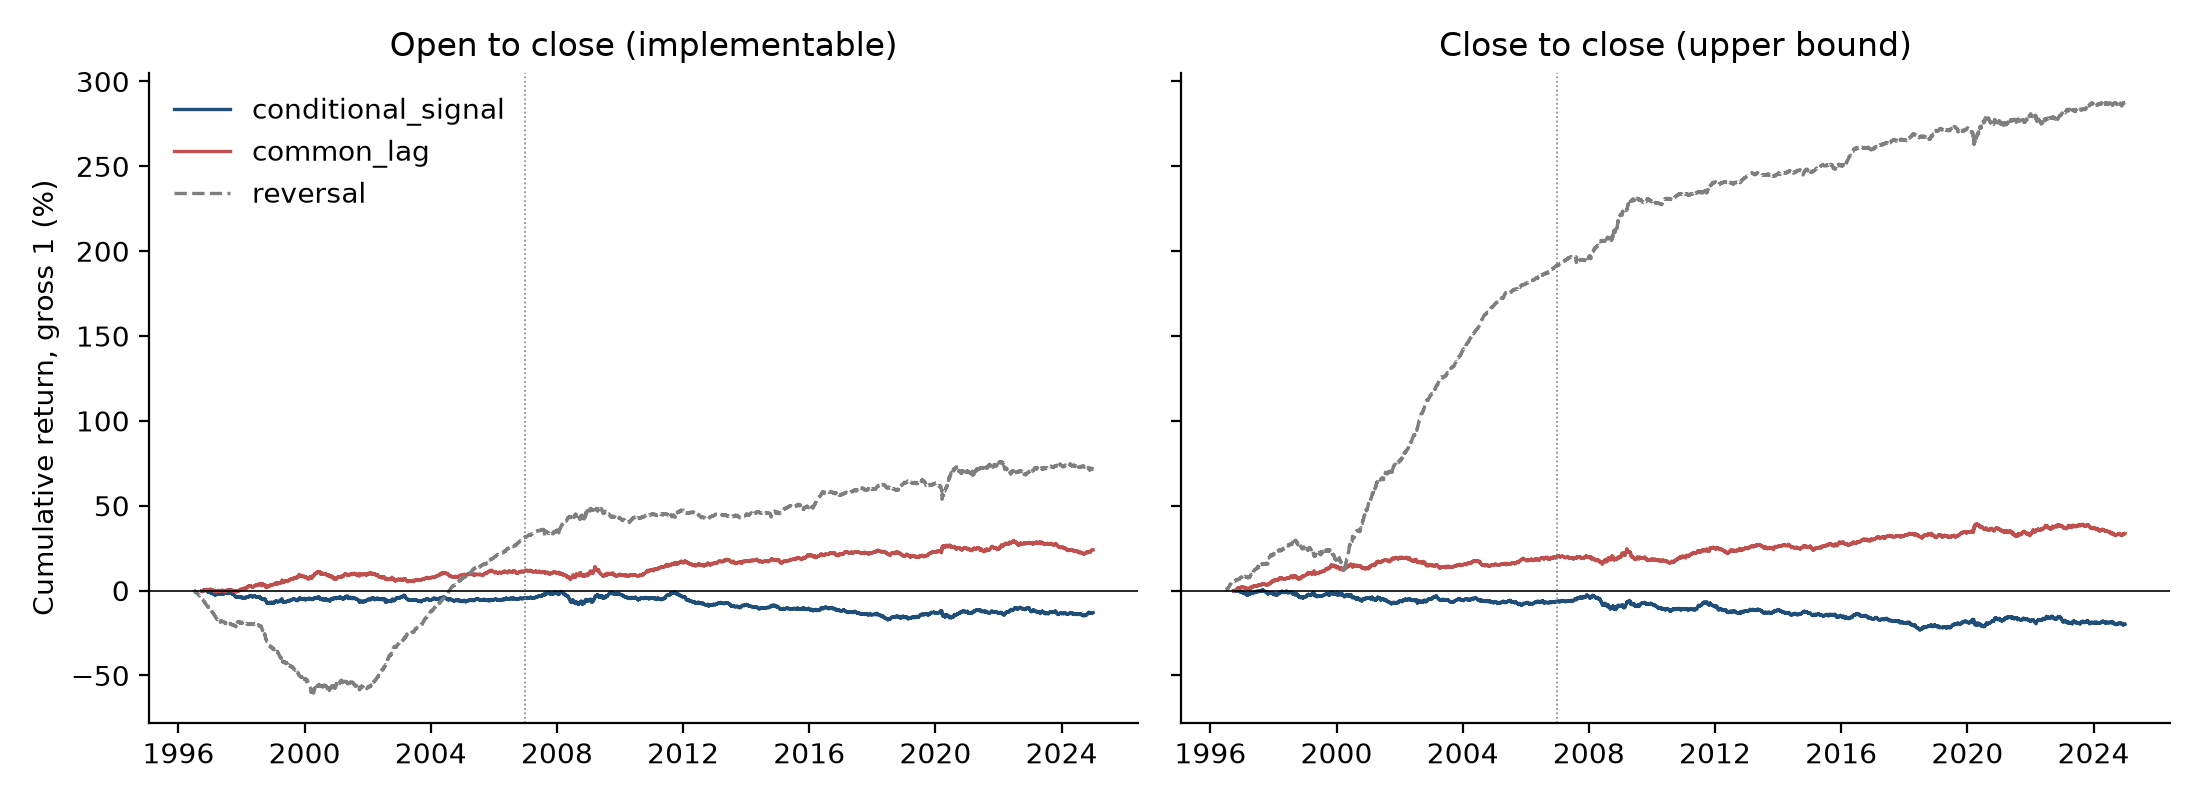
\includegraphics[width=0.92\textwidth]{p4_cumulative.png}
\caption{Cumulative return of the gross-1 books; the dotted line marks 2007.}\label{fig:cumulative}
\end{figure}



All code, result tables, figures and transcripts are in the project
repository:\\
\url{https://github.com/rezazamani2329/Equity-Market-UC-Berkeley_MFE/tree/main/Project_2_Conditional_Lead_Lag_Alpha}.
Table~\ref{tab:index} lists the result tables and figures by part. The design
documents are \file{docs/part4\_prereg.md} (pre-registration) and
\file{docs/part4\_deviations.md} (changes after the code audit).

\begin{table}[h]
\centering\footnotesize
\caption{Result tables and figures in the repository.}\label{tab:index}
\begin{tabularx}{\textwidth}{@{}>{\raggedright\arraybackslash}p{0.17\textwidth}YY@{}}
\toprule
Part & Tables (\file{results/}) & Figures (\file{figures/}) \\
\midrule
1. Data and baseline & \file{p1\_horizon\_profile.csv}, \file{p1\_coefficient\_by\_year.csv}, \file{p1\_bounce\_check.csv}, \file{p1\_universe\_attrition.csv} & \file{p1\_coefficient\_by\_year.png}, \file{p1\_quintile\_sort.png}, \file{p1\_horizon\_profile.png} \\
2. Shock decomposition & \file{p2\_conditional\_response\_horizon.csv}, \file{p2\_variance\_shares.csv} & \file{p2\_common\_vs\_shock.png}, \file{part2\_variance\_shares.png}, \file{part2\_leader\_robustness.png} \\
3. Signal validation & \file{p3\_horizon\_ic.csv}, \file{p3\_quintile\_spread\_h1.csv} & \file{p3\_ic\_by\_horizon.png}, \file{p3\_quintile\_monotonicity.png} \\
4. Portfolio and risk & \file{p4\_performance.csv}, \file{p4\_primary\_tests.csv}, \file{p4\_attribution.csv}, \file{p4\_costs.csv}, \file{p4\_var\_backtest.csv}, \file{p4\_stress.csv}, \file{p4\_decision.csv} & \file{p4\_cumulative.png}, \file{p4\_drawdown.png}, \file{p4\_timing\_decomposition.png} \\
5. Robustness & \file{p5\_net\_of\_cost.csv}, \file{p5\_yearly\_returns.csv}, \file{p5\_subperiods.csv}, \file{p5\_decision.csv} & \\
\bottomrule
\end{tabularx}
\end{table}

\clearpage
% ============================================================================
\section{Code}\label{app:code}
% ============================================================================

Each part has one script that regenerates its tables,
\file{scripts/run\_part1.py} to \file{run\_part5.py}, on the package in
\file{src/lead\_lag/}. The Part 5 cost calculation, from the Part 4 daily book
returns:

\begin{Verbatim}[fontsize=\footnotesize,frame=single,framesep=6pt]
# src/lead_lag/robustness/costs.py
ROUND_TRIP = 2.0  # traded notional per day of a gross-1 book that is flat overnight

def net_of_cost(gross, traded, cost_bp):
    """Daily return after a one-way cost of `cost_bp` basis points."""
    return gross - traded * cost_bp / 1e4

# scripts/run_part5.py: open-to-close books trade ROUND_TRIP x gross each day;
# close-to-close books are charged their realised turnover.
traded = {"C": ROUND_TRIP, "A": wide[(book, "turnover_carry")]}
s = summary_stats(net_of_cost(gross, traded[conv], cost))  # ann. mean, Newey-West t
\end{Verbatim}

The industry-book weights, from
\file{src/lead\_lag/portfolio/construction.py}: rank the industries on the
signal, demean, project out a constant, the industry's average follower beta
and its average previous-day follower return, split each industry's weight
equally across its followers, and scale to gross exposure 1.

% ============================================================================
\clearpage
\section{ChatGPT Interactions}\label{app:chatgpt}
% ============================================================================

The three interactions as recorded in the repository, in the files
\file{appendix/chatgpt\_p4.md} and \file{appendix/chatgpt\_p5.md}: exact prompts,
summaries, critical evaluation, and the full outputs.
\sloppy

\hypertarget{part-4-chatgpt-interactions}{%
\subsection{Part 4: ChatGPT interactions}\label{part-4-chatgpt-interactions}}

Two interactions, run on GPT-6.1 (sol, medium) on 2026-09-30, after the Part 4 design had
been pre-registered and the results computed. ChatGPT was therefore used as an
independent review of the design rather than to generate it. Each section gives the
exact prompt, a summary of the output, the critical evaluation, and what was adopted.
The full outputs are reproduced at the end of this file.

\begin{center}\rule{0.5\linewidth}{0.5pt}\end{center}

\hypertarget{interaction-1-robustness-design}{%
\subsubsection{Interaction 1: robustness design}\label{interaction-1-robustness-design}}

\hypertarget{prompt}{%
\paragraph{Prompt}\label{prompt}}

\begin{quote}
I am backtesting a daily-rebalanced long/short equity strategy on US stocks, 1996--2024,
using CRSP daily data. The universe is about 1,750 ``follower'' stocks a month, grouped
into 48 Fama-French industries. The signal is the previous day's return of each
industry's largest stock (the ``leader''), decomposed into a market-and-industry
component and a leader-specific component. Every follower in an industry gets the
same signal value. I trade at the close and hold one day.

List every way this backtest could show a profit that would not survive in real
trading, or that is not the effect I think I am measuring. For each one, say how I
would detect it in the data I have (CRSP daily prices, bid and ask, opening price,
volume, delisting returns, Fama-French daily factors) and what the fix is. Be
specific to this design rather than generic.
\end{quote}

\hypertarget{summary}{%
\paragraph{Summary}\label{summary}}

\begin{itemize}
\tightlist
\item
  About 70 failure modes in six groups (information timing, CRSP price artifacts,
  execution and shorting, delistings and accounting, alternative explanations,
  statistical inference), each with a detection method and a fix, ending with a
  seven-step priority order.
\item
  A fixed timing convention: with the leader's return on t−1, enter at the close of t,
  exit at the close of t+1, and earn the follower's return on t+1.
\item
  Stale follower prices and bid-ask bounce as the main mechanical explanations, to be
  checked by comparing close and midpoint returns and by splitting the holding-day
  return into overnight and daytime parts, with open entry as a test.
\item
  Because the signal is shared within an industry, the strategy is industry allocation:
  1,750 followers are not 1,750 independent forecasts, and industry neutrality would
  remove the payoff.
\item
  Market continuation, industry momentum and the follower being included in the
  industry index used to decompose the leader can all masquerade as leader information.
\end{itemize}

\hypertarget{critical-evaluation}{%
\paragraph{Critical evaluation}\label{critical-evaluation}}

\textbf{Where it was right, and matched what Part 4 found in the data}

\begin{itemize}
\tightlist
\item
  \textbf{Industry-level signal.} It said an industry-neutral book removes the payoff of a
  signal shared within an industry, and treated breadth as industry-days. That is the
  design fact Part 4's construction is built on.
\item
  \textbf{Market-beta timing.} Its ``generic market continuation'' item is what removes the
  conditional signal in Part 4: beta neutrality alone takes it from t = 3.0 to t = −0.6.
\item
  \textbf{Industry momentum and self-inclusion.} Its point that the industry factor contains
  the follower being predicted is the mechanism behind Part 4's finding that
  \texttt{common\_lag} is 0.63 correlated with the followers' own previous-day return.
\item
  \textbf{Calendar lag.} ``Lag on the common market calendar'' rather than the previous
  available observation is the defect the code audit found in the team's
  \texttt{lag\_leader\_components} (758 follower-days).
\item
  \textbf{Bounce and staleness.} The close-versus-midpoint comparison and the
  overnight/daytime split are exactly what show that about 80\% of the close-to-close
  reversal benchmark is bounce (10.1\% a year on closes against 1.9\% on midpoints) and that
  most of its close-to-close return arrives overnight (7.5 of 10.1 points a year; 15 of 18
  in 1996--2006).
\end{itemize}

\textbf{Where it was wrong or would have misled}

\begin{itemize}
\tightlist
\item
  \textbf{Its timing would have hidden the effect.} Our prompt said ``I trade at the close''.
  ChatGPT took that literally, correctly ruled out trading at the same close that produced
  the signal, and moved the trade to the close of t, a full session after the signal. That
  is a two-session gap, and Part 1 shows the effect is gone
  after one session, and in Part 4 every lead-lag book earns roughly nothing under this
  timing (\texttt{leader\_ret\_lag} t = 0.02). It did suggest testing entry at the next open and
  splitting the return into overnight and daytime parts, but it did not say that the next
  open is the earliest feasible entry and should be the headline. Part of the blame lies
  with our prompt: by stating the execution time, we steered it toward the wrong default.
\item
  \textbf{Too long and partly generic.} Many items do not apply here, were already handled
  by Part 1 (delisting repair, negative prices, split adjustment, point-in-time
  industry codes), or cannot be tested with this data (borrow availability, recalls,
  auction fills, margin ledgers, the Fama-French data vintage, which matters little when
  the factors are used only for attribution). The ten or so items that decide the result
  are buried among the rest; the closing priority list helps.
\item
  \textbf{No numbers on costs.} It cannot know the turnover, so it could only say costs might
  be decisive, not that the strategy is an order of magnitude below breakeven.
\end{itemize}

\textbf{Adopted.} Part 4 had already used open-to-close as its headline, the calendar lag and
the midpoint diagnostic, so the answer served as an independent check of those choices.
Its default close-to-close-of-t+1 timing was rejected for the reason above. Three checks
it suggests are not in Part 4 and are passed to Part 5: long and short legs reported
separately, P\&L concentration by industry and leader, and leave-one-industry-out tests.

\begin{center}\rule{0.5\linewidth}{0.5pt}\end{center}

\hypertarget{interaction-2-portfolio-construction-and-risk-model}{%
\subsubsection{Interaction 2: portfolio construction and risk model}\label{interaction-2-portfolio-construction-and-risk-model}}

\hypertarget{prompt-1}{%
\paragraph{Prompt}\label{prompt-1}}

\begin{quote}
I have a daily cross-sectional signal that takes one value per industry (48
industries) and is shared by every stock in that industry. I want a long/short book
that is dollar-neutral and market-beta-neutral, and that is also neutral to each
industry's average lagged stock return, so I isolate information that is not just
industry momentum. My only optimizer is scipy.

\begin{enumerate}
\def\labelenumi{\arabic{enumi}.}
\tightlist
\item
  Propose a construction, with the exact formula for the weights.
\item
  Propose a risk model suitable for this book and explain whether a diagonal
  (stock-specific) risk model is adequate.
\item
  Say how to set the position size: gross exposure versus a volatility target.
\item
  Give Python for the weights given a DataFrame with columns date, industry,
  signal, beta, own\_lag.
\end{enumerate}
\end{quote}

\hypertarget{summary-1}{%
\paragraph{Summary}\label{summary-1}}

\begin{itemize}
\tightlist
\item
  A covariance-weighted projection of the signal on the constraints (a constant, beta,
  and one industry-average own-lag variable):
  q = Σ⁻¹s − Σ⁻¹A(AᵀΣ⁻¹A)⁺AᵀΣ⁻¹s, scaled to the desired gross exposure.
\item
  Why 48 separate own-lag constraints, one per industry, or full industry-dollar
  neutrality would wipe out a signal shared within an industry.
\item
  A diagonal risk model is inadequate because net industry positions carry common
  industry risk; it recommends Σ = BFBᵀ + D with market, industry and style factors,
  shrunk and estimated on past data.
\item
  A volatility target with a gross-exposure cap, noting the target is missed when the
  cap binds, and holding zero when the projection removes nearly all of the signal.
\item
  Python implementing the projection with whitening and SVD rank handling.
\end{itemize}

\hypertarget{critical-evaluation-1}{%
\paragraph{Critical evaluation}\label{critical-evaluation-1}}

\begin{itemize}
\tightlist
\item
  \textbf{Agrees with Part 4 on the essentials.} One industry-level own-lag constraint rather
  than 48, a closed-form projection rather than an optimizer, and a diagonal model being
  inadequate.
\item
  \textbf{But it builds a different book, with a flaw it had itself warned about.} Its
  projection runs at the stock level on the raw signal, with each stock's own beta. With
  Σ = I, weights therefore vary within an industry and each industry's net weight grows with
  its number of followers, which is the ``follower count accidentally determines industry
  exposure'' problem it listed in its first answer. Part 4 instead ranks the industries,
  projects with each industry weighted equally, and splits each industry's weight equally
  across its followers.
\item
  \textbf{Its risk-model advice points to a real gap in Part 4.} It recommends a factor model
  (Σ = BFBᵀ + D) and calls a diagonal model inadequate. Part 4 has no full factor risk
  model; it sizes books by gross exposure and realized volatility instead. That does not change the
  verdict, since the books either lose money or earn far less than their costs, but it
  belongs in the limitations.
\item
  \textbf{One warning does not apply here.} It advises holding zero when the projection removes
  nearly all of the signal, while Part 4 always rescales to gross 1. On the real data the
  final weights of the pre-registered books keep a correlation of 0.61 (\texttt{common\_lag}) to
  0.88 (\texttt{shock\_lag}) with the signal, so the books are not trading a near-empty residual.
\item
  \textbf{It anticipated the volatility-target result.} Part 4's headline hits its 3× cap and
  realizes 6.7\% volatility rather than the 10\% target.
\item
  \textbf{Missed.} It did not mention that ordinary least-squares betas are biased down for
  thinly traded stocks, which is why Part 4 uses Dimson betas, and it projects the raw
  signal rather than ranks, which is more sensitive to outliers.
\item
  \textbf{Convention.} Its gross exposure of 2 means 100\% long and 100\% short; Part 4 reports
  books at gross 1 (50\% long, 50\% short), so its returns would be twice Part 4's for the
  same book.
\item
  \textbf{Code.} As copied, the code block lost its line breaks and the start of the function
  (signature, imports, date loop), so it cannot be run as is, and its statement that it
  verified the code cannot be checked from the transcript. Part 4 did not rely on it.
\end{itemize}

\textbf{Adopted.} No change to the pre-registered construction. The missing factor risk model
is added to the Part 4 limitations.

\begin{center}\rule{0.5\linewidth}{0.5pt}\end{center}

\hypertarget{reflection-report-section-3d}{%
\subsubsection{Reflection (report section 3d)}\label{reflection-report-section-3d}}

Used as an independent review after the design was fixed, ChatGPT was most useful as a
checklist. Its first answer worked out, without being told, the three issues that decide
Part 4: that a signal shared within an industry makes the strategy industry allocation (so
industry neutrality removes it), market-beta timing, and industry momentum leaking into
the ``common'' component through the industry index. It also flagged the calendar-lag defect
the code audit found. Its weakest point was timing: following our prompt's ``I trade at the
close'', it moved the trade a full session after the signal, a two-session gap,
and offered the next-open entry only as a test. That is partly a
lesson about our prompt, which should have asked for the earliest feasible execution rather
than stating one. It was long and partly generic, and it could not quantify costs. Its construction
answer shared Part 4's constraints but weighted industries by follower count, a problem it
had itself flagged, and its risk-model advice pointed to one genuine gap, the lack of a
full factor risk model. The pattern matches
HW1 and HW2: it is strong at listing what could go wrong and weak at judging which items
matter for a specific dataset.

\begin{center}\rule{0.5\linewidth}{0.5pt}\end{center}

\hypertarget{full-outputs}{%
\subsubsection{Full outputs}\label{full-outputs}}

\hypertarget{interaction-1-output}{%
\paragraph{Interaction 1 output}\label{interaction-1-output}}

The biggest risks in this design are \textbf{earning returns before your entry, trading stale follower prices, mistaking common-factor continuation for leader information, and treating 1,750 followers as independent signals}. Daily rebalancing also makes modest execution costs potentially decisive.

Below is a comprehensive audit of the material failure modes. Some can be diagnosed with your daily data; others can only be stress-tested. Historical borrow availability, auction fills, intraday quote timing, and the cause of a news shock cannot be established from these fields alone.

First, fix the time convention. Let \(r_{i,t}\) be the return from close \(t-1\) to close \(t\). \textbf{If you use the leader's return \(r_{L,t-1}\), enter at close \(t\), and exit at close \(t+1\), your earned follower return is \(r_{i,t+1}\).} The follower's \(r_{i,t}\) has already happened.

\textbf{1. Information timing and selection}

\begin{longtable}[]{@{}
  >{\raggedright\arraybackslash}p{(\columnwidth - 4\tabcolsep) * \real{0.3333}}
  >{\raggedright\arraybackslash}p{(\columnwidth - 4\tabcolsep) * \real{0.3333}}
  >{\raggedright\arraybackslash}p{(\columnwidth - 4\tabcolsep) * \real{0.3333}}@{}}
\toprule\noalign{}
\begin{minipage}[b]{\linewidth}\raggedright
Failure mode specific to your design
\end{minipage} & \begin{minipage}[b]{\linewidth}\raggedright
How to detect it
\end{minipage} & \begin{minipage}[b]{\linewidth}\raggedright
Fix
\end{minipage} \\
\midrule\noalign{}
\endhead
\bottomrule\noalign{}
\endlastfoot
\textbf{One-day return alignment error.} You use yesterday's leader return but credit today's follower close-to-close return despite entering today at the close. & For several trades, print signal start/end dates, order date, entry price, exit price, and the CRSP return date. Reconcile individual dollar profits manually. & Use the timeline above. Keep signal date, execution date, and return date as separate fields. \\
\textbf{Using the completed close to trade at that same close.} This can enter through leader returns, factor returns, volatility scaling, or follower weights---even if the headline signal is lagged. & Record the latest observation used by \emph{every} input. Compare against the order submission time, not merely the calendar date. & Freeze orders using information available before submission. Completed daily inputs generally require execution at a later opportunity. \\
\textbf{Fama--French factors treated as available immediately.} Yesterday's economic factor return and yesterday's published factor value are different objects. & Identify which factor files enter live signal construction and their assumed availability. Recompute with additional lags or internally constructed factors. Daily factor files do not establish historical publication times. & Construct contemporaneously available market/industry proxies yourself, or apply a defensible publication delay. Ex-post factors remain usable for attribution. \\
\textbf{Full-sample or forward-looking decomposition.} Leader betas, means, residual volatility, winsorization thresholds, or signal coefficients use future observations. & Recreate every day using a dataset truncated at the decision date. Compare signals with the original series. & Fit rolling or expanding models using past data only. A conservative specification estimates coefficients through the day before the return being decomposed. \\
\textbf{Month-end leader selection applied backward within the month.} The eventual largest stock can become leader partly because it rose during that month. & Compare the recorded leader with ranks at the previous month-end. Inspect leader changes and profit around them. & Select leaders using information available before the new month; hold that definition fixed for the stated selection period. \\
\textbf{Future-dependent follower eligibility.} Requiring complete monthly returns, positive volume throughout the month, survival, or a future exit quote selects favorable outcomes. & Compare your universe with eligibility reconstructed at each prior month-end. Examine excluded names' subsequent returns and delistings. & Set eligibility prospectively. Handle subsequent missing observations and trading failures inside the position ledger. \\
\textbf{Survivorship or endpoint selection.} Your historical 1,750-stock universe comes from stocks surviving to 2024 or a current list. & Examine entrants, exits, IPOs, and delisted stocks over time. Reconstruct membership from historical CRSP records. & Use point-in-time membership, retaining failed companies and securities that disappear. \\
\textbf{Historical industry assignment overwritten by current SIC.} Followers and leaders acquire relationships that did not exist then. & Compare assignments against effective-dated SIC histories; inspect reclassifications and mergers. Prices alone cannot validate this. & Use historical classification records. Distinguish ``FF48 SIC mapping'' from reproducing French's actual annual portfolio memberships. \\
\textbf{``Largest stock'' is misdefined.} Share price substitutes for market capitalization, shares have incorrect units, or one share class substitutes for the company. & Audit leader ranks using \(|PRC|\times SHROUT\), units, and company identifiers. Compare security-level and company-level ranks. & Define whether leadership is by security or company capitalization. For company leadership, aggregate eligible classes and specify which return represents the leader. You need historical shares and identifiers. \\
\textbf{Leader contamination among followers.} Another share class of the same company, or the leader itself, is traded as a follower. & Match leader and follower company identifiers; separately report affiliated-class profits. & Exclude the leader and, for an intercompany transmission claim, its other share classes. \\
\textbf{Identity/join errors.} Ticker reuse, many-to-many name-history joins, or merger links create duplicate trades or artificial continuity. & Require unique security--date rows; check row counts before and after joins and inspect abrupt identity changes. & Use permanent security identifiers and effective-dated joins; handle corporate events explicitly. \\
\textbf{``Previous day'' means previous available observation.} A suspended follower's next return spans several sessions but is labeled one day. & Measure trading-calendar gaps between observations and entry/exit records. & Lag on the common market calendar. Preserve gaps and actual elapsed holding periods. \\
\end{longtable}

French's published 48-industry portfolios use June assignments held from July through the following June, with a specified Compustat/CRSP SIC hierarchy. A monthly CRSP-SIC classification can be legitimate, but it is a different construction. \href{https://mba.tuck.dartmouth.edu/pages/faculty/ken.french/Data_Library/det_48_ind_port.html?utm_source=chatgpt.com}{Detail for 48 Industry Portfolios}

\textbf{2. CRSP prices and apparent lead--lag profits}

CRSP's legacy \texttt{PRC} can represent a trade price or a bid/ask average. Also, \texttt{BIDLO} and \texttt{ASKHI} are conditional bid/low and ask/high fields; they must not automatically be treated as executable quotes. Separate \texttt{BID} and \texttt{ASK} fields exist. \href{https://support.sas.com/documentation/cdl/en/etsug/63939/HTML/default/etsug_sasecrsp_sect017.htm?utm_source=chatgpt.com}{9.3}

\begin{longtable}[]{@{}
  >{\raggedright\arraybackslash}p{(\columnwidth - 4\tabcolsep) * \real{0.3333}}
  >{\raggedright\arraybackslash}p{(\columnwidth - 4\tabcolsep) * \real{0.3333}}
  >{\raggedright\arraybackslash}p{(\columnwidth - 4\tabcolsep) * \real{0.3333}}@{}}
\toprule\noalign{}
\begin{minipage}[b]{\linewidth}\raggedright
Failure mode
\end{minipage} & \begin{minipage}[b]{\linewidth}\raggedright
How to detect it
\end{minipage} & \begin{minipage}[b]{\linewidth}\raggedright
Fix
\end{minipage} \\
\midrule\noalign{}
\endhead
\bottomrule\noalign{}
\endlastfoot
\textbf{Negative \texttt{PRC} mishandled.} In legacy data the negative sign denotes a quote-based price, rather than a negative economic price. Sign changes can create enormous false returns. & Flag negative prices; inspect every large return against price signs and CRSP returns. & Use absolute price magnitudes for valuation while retaining the quote-price indicator. Prefer correctly interpreted CRSP return fields for total returns. \\
\textbf{Stale follower closes manufacture delayed reaction.} The liquid leader incorporates news while the follower's recorded last trade predates it; the next trade appears to ``follow.'' & Stratify profits by zero volume, repeated prices, zero-return runs, negative-price observations, lagged dollar volume, and spreads. Compare trade-close and genuine midpoint-return results. & Require prospectively adequate liquidity; model executable entry prices. Obtain timestamped quotes/trades for a definitive synchronization test. Positive daily volume does \textbf{not} prove a fresh closing trade. \\
\textbf{Bid--ask bounce masquerades as predictability.} Industry-wide buying/selling can affect which side supplies the follower close. & Compare close-return predictions with midpoint-return predictions on the same observations; measure close-minus-midpoint changes and next-day reversals. & Treat midpoints as a diagnostic valuation series, then price actual buys and sells appropriately. Do not claim midpoint profitability is executable profitability. \\
\textbf{Alternating trade and quote marks create returns without equivalent trades.} & Split profits into trade→trade, trade→quote, quote→trade, and quote→quote intervals. & Keep valuation and execution separate. A quote-derived mark is not evidence of an obtainable fill. \\
\textbf{Daily high/low fields used as spreads.} Your cost model or midpoint series actually uses the intraday range. & Inspect field names and definitions; compare candidate ``spreads'' with daily ranges and available true quotes. & Use genuine bid/ask fields. If unavailable, report cost scenarios rather than interpreting high/low ranges as quoted spreads. \\
\textbf{Bad, stale, or noncomparable quotes.} Crossed quotes, different adjustment bases, or noncontemporaneous observations distort midpoints and costs. & Flag nonpositive/crossed quotes, extreme relative spreads, repeated quotes, and large close--midpoint discrepancies; report coverage by exchange and year. & Apply documented quote-validity rules. Keep a separate matched-sample comparison so quote coverage does not silently change the universe. \\
\textbf{A split or distribution creates the leader signal.} Raw price changes are mistaken for economic returns, broadcasting a false shock to an entire industry. & Inspect large leader signals; compare raw-price returns with CRSP total and ex-distribution returns, where available. Check opening/closing adjustment consistency. & Use corporate-action-aware returns. Price, shares, volume, quotes, and opening prices must have consistent adjustment bases. \\
\textbf{Dividend price drops generate short profits.} The short earns the ex-dividend price decline without owing the dividend. & Compare price-return and total-return P\&L, especially around large price drops unexplained by market moves. Exact diagnosis needs return/distribution fields. & Include dividend receipts on longs and payments on shorts. Do not add distributions again if using total returns. \\
\textbf{Signal and traded P\&L use incompatible return definitions.} A dividend-inclusive leader return is interpreted as price information, or price-only follower returns are compared with total-return factors. & Re-run leader signals using price/ex-distribution and total returns; inspect distribution-sensitive dates. & State the economic return definition for each component; separate cash distributions from price news when testing transmission. \\
\textbf{Missing codes, percentage units, or exceptional observations become tradable signals.} One malformed leader observation affects every follower in its industry. & Check ranges and vendor missing-value codes; confirm FF percentage units versus CRSP decimal returns. Trace the largest industry-day P\&L contributions. & Parse missing values explicitly, validate units, and correct identifiable errors. Use any clipping threshold prospectively; do not delete genuine crashes merely because they are extreme. \\
\end{longtable}

Nonsynchronous observations can generate return autocorrelation and cross-autocorrelation. Thus, your largest-to-smaller-stock structure is particularly exposed to this alternative explanation; it is a hypothesis to test, not proof that all lead--lag profits are artificial. \href{https://www.nber.org/papers/w2960?utm_source=chatgpt.com}{NBER}

\textbf{3. Execution, costs, and the short book}

\begin{longtable}[]{@{}
  >{\raggedright\arraybackslash}p{(\columnwidth - 4\tabcolsep) * \real{0.3333}}
  >{\raggedright\arraybackslash}p{(\columnwidth - 4\tabcolsep) * \real{0.3333}}
  >{\raggedright\arraybackslash}p{(\columnwidth - 4\tabcolsep) * \real{0.3333}}@{}}
\toprule\noalign{}
\begin{minipage}[b]{\linewidth}\raggedright
Failure mode
\end{minipage} & \begin{minipage}[b]{\linewidth}\raggedright
How to detect or bound it with your data
\end{minipage} & \begin{minipage}[b]{\linewidth}\raggedright
Fix
\end{minipage} \\
\midrule\noalign{}
\endhead
\bottomrule\noalign{}
\endlastfoot
\textbf{CRSP's close is assumed to be your closing-auction fill.} A last reported trade can be a different execution opportunity. & Identify reliance on quote-based/no-volume closes; compare close-entry results with delayed open-entry results. Daily data cannot establish auction accessibility or depth. & Use the close as an explicitly conditional benchmark; validate auction fills with auction/intraday data or actual executions. \\
\textbf{Profitable adjustment happens before your delayed fill.} The follower catches up overnight or immediately at the opening. & For the correctly aligned holding day, split adjusted price returns into close→open and open→close. Also test next-open entry through the following close. & Report exactly which interval earns the profit and whether your order could precede it. An open-entry strategy cannot collect the preceding gap. \\
\textbf{Free crossing of the spread.} Frequent industry sign changes cause followers to trade in the same direction together. & Calculate costs on actual net dollar trades using valid relative spreads. Stress multiple spread assumptions and report gross versus net results. & Charge buys at ask/sells at bid under a marketable-order model, or use a defensible auction model. Spread crossing is not automatically the right model for genuine auction fills. \\
\textbf{Passive fills assumed whenever favorable.} Trading at the midpoint or bid/ask is treated as guaranteed. & Compare optimistic midpoint/passive P\&L with aggressive-fill scenarios. Daily prices cannot reveal fill probability or adverse selection. & Do not award guaranteed spread capture. Validate a passive strategy with order-level data. \\
\textbf{Commissions, fees, and trading frictions omitted.} Low gross daily returns can disappear even without much impact. & Report net traded dollars, ticket counts, and break-even total cost per traded dollar, by period. & Apply historically relevant schedules or transparent cost ranges, including minimum-ticket effects where material. \\
\textbf{Turnover calculated from yesterday's targets rather than today's actual holdings.} Returns, cash flows, and membership changes alter the portfolio before rebalancing. & Reconcile positions immediately before each trade with target positions. Include monthly additions/removals and sign flips. & Trade from drifted holdings. Net retained positions rather than automatically closing/reopening them; charge a long-to-short flip for the full change in shares. \\
\textbf{Unlimited liquidity and capacity.} Simultaneous follower orders overwhelm small stocks even if aggregate capital appears modest. & For several AUM levels, compute order dollars/lagged average dollar volume, largest participation, and contribution from constrained names. Inspect industry-wide order concentration. & Cap positions and participation using prior information; model nonlinear impact. Total daily volume is only a loose capacity bound for close execution. \\
\textbf{Same-day volume determines achievable size.} Realized full-day volume or the best eventual liquidity day enters sizing. & Recompute sizes using trailing volume available before orders. & Use lagged liquidity forecasts; model partial fills without knowledge of subsequent volume. \\
\textbf{Free and universal stock borrowing.} The short followers may be precisely the small/distressed names with expensive or unavailable borrow. & Separate long and short contributions; stratify shorts by lagged price, volume, spreads, and distress proxies. Apply borrow-fee and unavailable-name scenarios. & Obtain historical lending data for validation. Otherwise report conditional net returns and transparent borrow scenarios; liquidity is not proof of borrow availability. \\
\textbf{Recalls, buy-ins, short-sale restrictions, or emergency bans ignored.} & Identify short profits concentrated in distress/crisis episodes and stress forced covering or short exclusions. Daily CRSP cannot identify actual locates or restricted execution opportunities. & Use historical restriction/borrow records and operational rules. Do not infer unrestricted short execution from a recorded price. \\
\textbf{Halts and disappearing stocks conveniently liquidate at their last mark.} & Inspect positions with missing exit prices, zero volume, large observation gaps, and delistings. Check whether they vanish from P\&L. & Keep positions open until a feasible exit or terminal settlement; model capital tied up and delayed liquidation. \\
\textbf{Cash, financing, collateral, and margin create fictitious extra return.} Short proceeds are treated as freely investable cash, or financing is ignored. & Reconcile equity, gross exposure, long funding, short collateral, cash balances, interest, and losses each day. & Use an explicit broker cash/margin ledger. RF alone is not the actual funding or short-rebate rate. Include liquidation when equity/margin constraints bind. \\
\textbf{Weekend and holiday costs understated.} ``One day'' actually includes several calendar days. & Compare funding/borrow accrual with calendar time between entry and exit. & Accrue applicable financing and borrow costs over elapsed calendar days. \\
\end{longtable}

\textbf{4. Delistings and portfolio accounting}

\begin{longtable}[]{@{}
  >{\raggedright\arraybackslash}p{(\columnwidth - 4\tabcolsep) * \real{0.3333}}
  >{\raggedright\arraybackslash}p{(\columnwidth - 4\tabcolsep) * \real{0.3333}}
  >{\raggedright\arraybackslash}p{(\columnwidth - 4\tabcolsep) * \real{0.3333}}@{}}
\toprule\noalign{}
\begin{minipage}[b]{\linewidth}\raggedright
Failure mode
\end{minipage} & \begin{minipage}[b]{\linewidth}\raggedright
Detection
\end{minipage} & \begin{minipage}[b]{\linewidth}\raggedright
Fix
\end{minipage} \\
\midrule\noalign{}
\endhead
\bottomrule\noalign{}
\endlastfoot
\textbf{Delisting losses omitted, or short gains overstated.} Terminal economic returns disappear with the security. & Match every held disappearing security to delisting information; reconcile its last ordinary return, terminal return, and position. & Include terminal economics on both sides. For legacy, nonoverlapping ordinary and delisting return segments compound as \((1+RET)(1+DLRET)-1\); they are not simply added. \\
\textbf{Delisting return counted twice or booked at an impossible cash date.} & Audit your CRSP format and return coverage; inspect every terminal position and settlement date. & Check whether terminal effects are already incorporated before applying another adjustment. Separate economic valuation from actual receipt/payment of cash. \\
\textbf{Missing delisting returns replaced by zero, or unfavorable terminal rows discarded.} & Tabulate missing terminal returns and show P\&L under alternative terminal-payoff assumptions, separately for longs/shorts. & Use documented, event-sensitive assumptions and sensitivity ranges. Exact recovery requires additional terminal-event data. \\
\textbf{Held stocks with missing returns are dropped and weights renormalized after the fact.} & Compare the position list before the holding period with the names included in its return denominator. & Preserve all positions and cash. A missing observation is a valuation/execution problem, not permission to redistribute capital retrospectively. \\
\textbf{Returns use ending weights or realized winners receive more weight.} & Reconstruct profits from entry shares, actual prices, and distributions; compare with the weighted-return calculation. & Use beginning-of-period exposures. Lag capitalization and volatility inputs appropriately. \\
\textbf{Return denominator exaggerates performance.} \(R_L-R_S\) is advertised as the return on a 100\% gross portfolio. & Report long dollars, short dollars, gross/net exposure, equity, and P\&L together. & For 50\% long and 50\% short relative to equity, contribution is \(0.5R_L-0.5R_S\). A 100\% long/100\% short book has 200\% gross exposure. State the convention. \\
\textbf{Short returns compounded incorrectly.} Inverting a stock wealth index is substituted for daily short P\&L; negative equity or \textgreater100\% short losses are ignored. & Reconcile individual shorts in large rallies and verify portfolio equity never receives impossible resets. & Use signed shares and dollar P\&L. Apply actual collateral and solvency constraints. \\
\textbf{Daily arithmetic profits, overlapping sleeves, or leverage resets misstate investable wealth.} & Compound the daily equity ledger and compare with reported annual returns; check that capital is not reused across overlapping holdings. & Report a funded, self-financing wealth path with costs and cash flows. Geometric wealth growth differs from annualized mean return. \\
\end{longtable}

Factor-file vintage also deserves an audit: French switched the production source from legacy FIZ to CIZ beginning with the January 2025 release. Freeze and identify your CRSP and factor vintages rather than silently mixing revised histories. \href{https://mba.tuck.dartmouth.edu/pages/faculty/ken.french/data_library.html?utm_source=chatgpt.com}{Data Library}

\textbf{5. Profits that may be real but measure something else}

Suppose you write the leader's excess return as

\[
r^e_{L,g,d}
=\widehat\alpha_{g,d}
+\widehat\beta_{M,g,d}M_d
+\widehat\beta_{I,g,d}I_{g,d}
+\widehat\varepsilon_{L,g,d}.
\]

The residual is \textbf{specific to this statistical model}, not established leader-specific news. Orthogonality in an estimation sample does not establish causal independence or remove all future factor exposure.

\begin{longtable}[]{@{}
  >{\raggedright\arraybackslash}p{(\columnwidth - 4\tabcolsep) * \real{0.3333}}
  >{\raggedright\arraybackslash}p{(\columnwidth - 4\tabcolsep) * \real{0.3333}}
  >{\raggedright\arraybackslash}p{(\columnwidth - 4\tabcolsep) * \real{0.3333}}@{}}
\toprule\noalign{}
\begin{minipage}[b]{\linewidth}\raggedright
Alternative explanation
\end{minipage} & \begin{minipage}[b]{\linewidth}\raggedright
Detection using your data
\end{minipage} & \begin{minipage}[b]{\linewidth}\raggedright
Fix or appropriate interpretation
\end{minipage} \\
\midrule\noalign{}
\endhead
\bottomrule\noalign{}
\endlastfoot
\textbf{Generic market continuation or market timing.} Leaders proxy for yesterday's market move, while long and short industries have different betas. & Compare with a market-only signal; estimate rolling portfolio market exposure and regress realized strategy returns on contemporaneous FF factors. Test lagged market predictors of followers. & Report the market-driven component separately. Construct ex-ante beta-controlled portfolios and assess the remaining incremental leader signal. \\
\textbf{Industry continuation rather than leader transmission.} & Compare against lagged industry returns constructed without the leader; include both industry and leader residual predictors. & Require incremental out-of-sample prediction beyond the industry benchmark. Otherwise describe industry timing. \\
\textbf{The industry factor contains the leader being decomposed.} Its large weight mechanically determines how much of its own return is assigned to the common component. & Measure leader weight in the industry portfolio; rebuild the factor excluding the leader company and compare decompositions. & Use a leave-leader-out industry benchmark for identification. Report sensitivity to equal/value weighting. Inclusion is not automatically look-ahead, but it changes the meaning of the decomposition. \\
\textbf{The factor contains the follower being predicted.} Follower own-return information enters the purported leader signal through residualization. & For each follower, remove that follower from the industry factor; compare results. Alternatively use a disjoint reference set of stocks. & Use leave-follower-out or disjoint benchmark portfolios where feasible; show that self-inclusion does not explain results. \\
\textbf{Industry weights/membership use contemporaneous or future information.} & Rebuild industry returns with beginning-of-period weights and prospective membership; compare signals. & Lag portfolio weights and define membership prospectively. \\
\textbf{Omitted common factors are called leader-specific.} Size, value, profitability, investment, momentum, liquidity, or subindustry news remain in the residual. & Add available FF factors and momentum if separately available; add returns of other large peers and CRSP-built liquidity/size portfolios. Compare residuals and incremental forecasts. & Label the residual conditional on the model used. Test richer models prospectively; recognize that your data cannot exhaust all economic shocks. \\
\textbf{Market and industry are collinear; attribution is unstable.} & Track condition numbers, coefficient instability, residual variance, and component correlations. Compare joint regression with alternative sequential decompositions. & Define the projection convention explicitly. Orthogonalizing industry to market gives an ordered interpretation, not a uniquely true allocation. \\
\textbf{Leader coefficients change through time.} Stale betas leave common shocks in the ``specific'' term, especially in crises or after business changes. & Check rolling residual--factor correlations, breakpoints, and forecast performance around leader switches. & Use past-only rolling/shrunk estimates and sensible minimum-history requirements; report window sensitivity. \\
\textbf{Follower own momentum/reversal explains the forecast.} A shared shock links yesterday's leader return to follower returns already observed. & Control for follower returns over the signal day and intervening day, prior momentum, lagged liquidity, and volatility. Compare with a follower-only predictor. & Demonstrate incremental prediction beyond what followers already reveal before entry. Keep these controls available at decision time. \\
\textbf{A large-stock/liquidity effect is mistaken for an industry relationship.} & Replace the leader with size/liquidity-matched stocks from other industries; compare the largest, second-largest, and a large-peer portfolio. & Require stronger prediction within the assigned industry than from comparable outsiders and broader large-stock benchmarks. \\
\textbf{Common news timing creates apparent leadership without transmission.} Both companies react to the same event at different times; broad SIC groups hide subindustry shocks. & Test industry specificity, peer-return controls, lead/reverse-lead patterns, and opening versus daytime responses. Inspect extreme event dates. & Describe predictive ordering unless news timestamps or another identification design supports causal transmission. Daily returns cannot establish who learned from whom. \\
\textbf{Mechanical same-industry positions create an industry allocation strategy.} Because every follower gets the same signal, trading more followers does not add distinct stock-selection information. & Aggregate weights and P\&L to industry-day observations. Compare with a strategy trading follower industry baskets directly. & Report industry-level exposures and breadth. Describe the strategy as industry allocation based on leaders, with stock-level implementation. \\
\textbf{Follower count accidentally determines industry exposure.} An industry with 150 names receives much more capital than one with 10 under equal stock weights. & Compare industry weights with follower counts; run equal-industry, equal-stock, and capitalization/liquidity-weighted variants. & Choose and state the intended exposure rule. Separate signal quality from the incidental number of listed followers. \\
\textbf{Long/short or residual signals are mistaken for industry neutrality.} & Inspect each industry's net dollar and beta exposure. & Do not claim industry neutrality. With identical signals and equal factor sensitivities within an industry, imposing zero net industry exposure removes the common-signal payoff; any remaining payoff comes from differing weights/exposures. \\
\textbf{Stock-level ranking ties produce unintended selection.} Every follower in an industry has the same score, but stock quantiles cut through ties using ticker, row order, or another hidden rule. & Shuffle row order and re-sort; examine industries split across long/short cutoffs. & Rank industries or use explicit, deterministic allocation across tied stocks. Report any secondary selection variable. \\
\textbf{Separate component portfolios give misleading attribution.} Ranking, volatility scaling, and constraints are nonlinear, so common-component and residual-component portfolio profits need not add to total-signal profit. & Compare score additivity with actual position additivity; fit both predictors jointly and compare nested forecasts. & Separate predictive attribution from implementable portfolio comparisons. Do not present nonlinear portfolio P\&Ls as an additive decomposition. \\
\textbf{Contemporaneous controls either manufacture or remove the result.} Realized holding-period factors are used to form positions, or industry returns containing followers absorb the outcome being explained. & Distinguish executable P\&L, ex-post risk regression, and predictive regression; audit dates and factor constituents. & Use future returns only as outcomes or clearly labeled attribution controls. Use independent industry benchmarks where outcome overlap matters. \\
\end{longtable}

\textbf{6. Statistical confidence and historical relevance}

\begin{longtable}[]{@{}
  >{\raggedright\arraybackslash}p{(\columnwidth - 4\tabcolsep) * \real{0.3333}}
  >{\raggedright\arraybackslash}p{(\columnwidth - 4\tabcolsep) * \real{0.3333}}
  >{\raggedright\arraybackslash}p{(\columnwidth - 4\tabcolsep) * \real{0.3333}}@{}}
\toprule\noalign{}
\begin{minipage}[b]{\linewidth}\raggedright
Failure mode
\end{minipage} & \begin{minipage}[b]{\linewidth}\raggedright
Detection
\end{minipage} & \begin{minipage}[b]{\linewidth}\raggedright
Fix
\end{minipage} \\
\midrule\noalign{}
\endhead
\bottomrule\noalign{}
\endlastfoot
\textbf{Pseudoreplication: 1,750 identical industry signals appear to be 1,750 independent forecasts.} & Compare stock-level standard errors with industry-day aggregation; examine residual correlation within industries and across the same date. & For prediction panels, account for dependence across dates and industries using appropriate clustering/block inference. For strategy returns, use the daily portfolio series with serial-dependence-aware inference. \\
\textbf{Generated residual uncertainty is ignored.} Estimated leader betas are treated as known observations. & Re-estimate the decomposition inside resampling and compare confidence intervals. & Resample time blocks and rerun estimation, signal construction, and portfolio formation---not just the final residual regression. \\
\textbf{Multiple testing selects the profitable version.} Two components, signs, windows, filters, weighting rules, industries, and start dates create many opportunities. & Keep an inventory of all tried specifications; compare the selected version with untouched periods. & Use chronological training/validation/test partitions and nested walk-forward selection; adjust inference for the actual search. \\
\textbf{Random train/test splits leak regimes and repeated signals.} Followers sharing the same industry-day shock land in both sets. & Inspect whether the same dates or industry-day signals occur in training and test sets; check overlapping labels/windows. & Split chronologically, with an appropriate gap for overlapping outcomes. Fit all transformations within training windows. \\
\textbf{A few leaders, industries, or days explain the result.} & Report P\&L by leader, industry, year, long/short side, and the largest contributing days. Run leave-one-industry/leader-out tests and contiguous-block exclusions. & Report concentration and robust uncertainty. Do not retrospectively delete economically valid events to obtain a preferred result. \\
\textbf{Older market structure drives the pooled average.} A profitable 1990s lag disappears in modern liquid trading. & Show gross/net performance, spreads, staleness, and turnover by era; test later periods under a frozen specification. & Base a current tradability claim on recent, genuinely held-out results and relevant costs. Historical existence is a separate claim. \\
\textbf{Calendar seasonality or crisis exposure supplies the premium.} Industry signals coincide with month-end moves, holiday intervals, or crisis risk. & Break out month-end, weekday, holiday-gap, and high-volatility results; examine factor exposures and downside conditional on market states. & Report conditional performance and risk; test incremental predictive value beyond calendar/state controls available before trading. \\
\textbf{Sharpe and t-statistics ignore serial dependence, tails, or changing leverage.} & Examine autocorrelation, drawdowns, skew, tail losses, gross exposure, and rolling performance; compare naive and block/HAC inference. & Use net funded returns, serial-dependence-aware uncertainty, and tail/drawdown reporting. A high annualized daily Sharpe alone is insufficient. \\
\textbf{Placebos accidentally preserve or destroy the wrong structure.} Stock-level randomization breaks the industry shock dependence and makes your result look exceptional. & Compare industry-label permutations, matched outsider leaders, reverse direction, and blockwise date shifts. & Preserve the dependence relevant to each null. Treat placebos as complementary tests, not proof of causality. \\
\end{longtable}

I would prioritize these checks in this order:

\begin{enumerate}
\def\labelenumi{\arabic{enumi}.}
\tightlist
\item
  \textbf{Manually reconcile the signal/entry/exit timeline and several trades}, including a short, a dividend date, a gap, and a delisting.
\item
  \textbf{Rebuild all signals and monthly selections prospectively}, with past-only decomposition estimates.
\item
  \textbf{Compare close and genuine-midpoint results on an identical sample}, then stratify by staleness, spreads, and liquidity.
\item
  \textbf{Split the earned holding-day return into overnight and daytime components}, and test delayed open execution.
\item
  \textbf{Calculate net P\&L from drifted holdings}, including realistic spread/auction assumptions, capacity, borrow, and financing scenarios.
\item
  \textbf{Test incremental leader-residual prediction against market, leave-leader-out industry, follower-own-return, and matched-outsider benchmarks.}
\item
  \textbf{Evaluate at industry-day and daily-portfolio levels}, with chronological out-of-sample testing and dependence-aware inference.
\end{enumerate}

The defensible outcome is three separate findings: \textbf{predictive ordering in recorded daily returns}, \textbf{incremental prediction beyond available common and follower information}, and \textbf{profit under feasible execution and funding}. Passing one does not establish the other two.

\hypertarget{interaction-2-output}{%
\paragraph{Interaction 2 output}\label{interaction-2-output}}

Use a covariance-weighted projection of the signal onto your neutrality constraints. But first distinguish one industry-momentum exposure from 48 separate constraints: the latter generally destroy your industry-level signal.

\begin{enumerate}
\def\labelenumi{\arabic{enumi}.}
\tightlist
\item
  Construction and exact weights
\end{enumerate}

For a given date, define:
\[ s_i=s_{g(i)},\qquad m_g=\frac{1}{n_g}\sum_{i:g(i)=g}\mathrm{own\_lag}_i, \qquad m_i=m_{g(i)}. \]
Here, \(m_i\) is the industry-average lagged return broadcast back to each stock. I assume an equal-weighted average over your eligible universe.
The useful neutrality conditions are:
\[ \mathbf1^\top w=0,\qquad \beta^\top w=0,\qquad m^\top w=0. \]
The last condition neutralizes one cross-sectional industry-momentum variable. It does not require each industry to have zero net investment.
Set \(A=[\mathbf1,\beta,m]\), and let \(\Sigma\) be a positive-definite daily stock-return covariance estimate. Solve
\[ \max_q\left\{s^\top q-\frac12q^\top\Sigma q\right\} \quad\text{subject to }A^\top q=0. \]
The exact solution is
\[ \boxed{ q=\Sigma^{-1}s- \Sigma^{-1}A \left(A^\top\Sigma^{-1}A\right)^+ A^\top\Sigma^{-1}s } \]
where \(+\) denotes the Moore--Penrose pseudoinverse, allowing redundant constraints.
For gross exposure \(G\),
\[ \boxed{w=G\,\frac{q}{\sum_i|q_i|}}. \]
Weights are fractions of NAV. Thus \(G=2\) means 100\% long and 100\% short. Scaling preserves all three neutralities. This is a risk-adjusted direction normalized to gross; it is not generally the solution to maximizing raw signal under an \(L^1\) constraint.
Why 48 separate momentum constraints fail: write \(W_g=\sum_{i\in g}w_i\). If you impose
\[ m_gW_g=0\quad\text{separately for every }g, \]
then every industry with \(m_g\ne0\) must have \(W_g=0\). Consequently,
\[ s^\top w=\sum_g s_gW_g=0. \]
Within-industry long/short positions may remain feasible, but your shared industry signal cannot predict their return. Full industry-dollar neutrality has the same problem.
Also, \(m^\top w=0\) removes linear exposure to this particular momentum control; it does not establish that the remaining signal represents distinct information. If you also want stock-level reversal neutrality, append individual \texttt{own\_lag} to \(A\).

\begin{enumerate}
\def\labelenumi{\arabic{enumi}.}
\setcounter{enumi}{1}
\tightlist
\item
  Risk model
\end{enumerate}

Use a factor model containing market, industry, and relevant style risks:
\[ r=Bf+\epsilon,\qquad \boxed{\Sigma=BFB^\top+D}. \]
Include your market betas, industry indicators, and estimated style exposures such as size, value, and momentum. Estimate factor covariance \(F\) with shrinkage and specific variances \(D\) with positive floors, using only history available before trading. Specify industry factors consistently with the market factor---for example, use market-residualized industry returns. Factor models provide both a parsimonious covariance estimate and a decomposition into common and specific risk. \href{https://docs.mosek.com/portfolio-cookbook/factormodels.html?utm_source=chatgpt.com}{MOSEK Portfolio Optimization Cookbook 1.6.0}
A stock-specific diagonal model alone is generally inadequate for this book. Its industry net positions carry common industry risk. For industry covariance \(F_{\mathrm{ind}}\), that contribution is
\[ W^\top F_{\mathrm{ind}}W. \]
Adding more stocks within an industry diversifies specific risk, but does not eliminate this term. A diagonal model falsely treats those stocks as independent and can encourage excessive industry exposure.
Diagonal risk can be adequate if the omitted common-factor exposures are zero or negligible. Your momentum constraint does not ensure that. Market-beta neutrality cancels the modeled market exposure, while industry and style risks remain.

\begin{enumerate}
\def\labelenumi{\arabic{enumi}.}
\setcounter{enumi}{2}
\tightlist
\item
  Position size
\end{enumerate}

Use a volatility target with a gross-exposure cap when managing risk. Fixed gross is useful for comparing signals under consistent leverage, but does not give consistent volatility.
For annual target \(\sigma_*\), with daily covariance \(\Sigma\),
\[ \boxed{ w=cq,\qquad c=\min\left( \frac{\sigma_*}{\sqrt{252\,q^\top\Sigma q}}, \frac{G_{\max}}{\sum_i|q_i|} \right). } \]
The volatility target will be missed when the gross cap binds. The \(\sqrt{252}\) annualization assumes negligible serial covariance; check realized strategy volatility.
Do not leverage a numerically tiny residual after projection: hold zero when the constraints remove essentially all signal. Use position, industry, liquidity, and turnover limits in a production optimizer; clipping weights afterward breaks neutrality.

\begin{enumerate}
\def\labelenumi{\arabic{enumi}.}
\setcounter{enumi}{3}
\tightlist
\item
  Python
\end{enumerate}

This implements both interpretations, handles redundant constraints through SVD, and preserves row order. With only your five columns, it can construct weights using an identity risk penalty. Those columns are insufficient to estimate a realistic covariance or support volatility targeting, so supply a covariance callback for that.

\emph{(The code block below lost its line breaks and its opening lines when copied from ChatGPT; it is reproduced as copied.)}

\begin{verbatim}
import numpy as np            codes, labels = g["industry"].factorize(sort=False)            H = np.eye(len(labels))[codes]            controls = H * m[:, None]        A = np.column_stack([np.ones(n), beta, controls])        C = (            np.ones(n)            if covariance is None            else np.asarray(covariance(date, g), dtype=float)        )        if not np.isfinite(C).all():            raise ValueError(f"Nonfinite covariance on {date}.")        # Sigma = L L.T. Project in whitened coordinates.        if C.shape == (n,):            if np.any(C <= 0):                raise ValueError("Diagonal variances must be positive.")            root = np.sqrt(C)            y = s / root            X = A / root[:, None]            def unwhiten(v):                return v / root            def variance(v):                return np.dot(C, v * v)        elif C.shape == (n, n):            if not np.allclose(C, C.T, rtol=1e-10, atol=1e-12):                raise ValueError("Covariance must be symmetric.")            L = cholesky((C + C.T) / 2, lower=True)            y = solve_triangular(L, s, lower=True)            X = solve_triangular(L, A, lower=True)            def unwhiten(v):                return solve_triangular(L.T, v, lower=False)            def variance(v):                return v @ C @ v        else:            raise ValueError("Covariance has an incorrect shape.")        # Normalize control columns before rank determination.        norms = np.linalg.norm(X, axis=0)        keep = norms > 0        X = X[:, keep] / norms[keep]        U, singular, _ = svd(X, full_matrices=False)        U = U[:, singular > rcond * singular[0]]        residual = y - U @ (U.T @ y)        if np.linalg.norm(residual) <= rcond * np.linalg.norm(y):            continue  # No surviving signal; leave weights at zero.        q = unwhiten(residual)        scale = gross / np.abs(q).sum()        if target_vol is not None:            annual_vol = np.sqrt(252 * variance(q))            scale = min(scale, target_vol / annual_vol)        weights[pos] = scale * q    out["weight"] = weights    return out
\end{verbatim}

Usage:

\begin{verbatim}
# Weight construction from the supplied columns; identity penalty.book = make_weights(df, gross=2.0)# Recommended: realistic daily covariance, 10% annual vol, 200% gross cap.book = make_weights(    df,    covariance=lambda date, g: daily_covariance(date, g),    target_vol=0.10,    gross=2.0,)
\end{verbatim}

I verified the projection against the closed-form formula, including neutrality, gross scaling, redundant constraints, and signal annihilation under separate industry constraints.


\clearpage
\hypertarget{part-5-chatgpt-interaction}{%
\subsection{Part 5: ChatGPT interaction}\label{part-5-chatgpt-interaction}}

One interaction, run on ChatGPT on 2026-10-03, after Part 4's results were final and
before any Part 5 result was computed. ChatGPT was therefore used to
design the Part 5 tests and to fix their pass/fail rules in advance, rather than to review
results already in hand. The section below gives the exact prompt, a summary of the output,
the critical evaluation, and what is adopted. The full output is reproduced at the end of
this file.

\begin{center}\rule{0.5\linewidth}{0.5pt}\end{center}

\hypertarget{interaction-3-robustness-design-for-costs-microstructure-and-out-of-sample-tests}{%
\subsubsection{Interaction 3: robustness design for costs, microstructure and out-of-sample tests}\label{interaction-3-robustness-design-for-costs-microstructure-and-out-of-sample-tests}}

\hypertarget{prompt}{%
\paragraph{Prompt}\label{prompt}}

\begin{quote}
I am finishing the robustness section of a daily long/short US equity backtest,
1996--2024, on CRSP daily data. About 1,750 ``follower'' stocks a month sit in 48
Fama-French industries. The signal is the previous day's return of each industry's
largest stock (the ``leader''), split into a market-and-industry component and a
leader-specific component; every follower in an industry gets the same value. The
books are built at the industry level, neutral to dollar, market beta and the
industry's own lagged return, with gross exposure 1 (50\% long, 50\% short). They are
formed from information at the previous close, bought at the open and sold at that
day's close.

Results so far: before costs the books earn between −0.5\% and +0.9\% a year. Because
they are flat overnight they trade twice their gross every day. Over 2007--2024 the
one-way cost at which each book's return is zero is under 0.2 bp, against a median
quoted half-spread of 2.6 bp for the stocks held. The return is concentrated in
1996--2006. The whole sample has already been examined and no holdout was reserved.
Our current conclusion is ``do not implement''.

Data I have: CRSP daily open, close, closing bid and ask, volume, shares outstanding
and delisting returns; Fama-French daily factors; and one-minute best bid and offer
by exchange (not consolidated) for 1,209 of the stocks, May 2018 to December 2024.

\begin{enumerate}
\def\labelenumi{\arabic{enumi}.}
\tightlist
\item
  Propose a transaction cost model with the exact formula for cost per stock per
  day, covering spread, market impact as a function of trade size relative to
  volume, and trading in the opening and closing auctions. Say which components I
  can calibrate from this data, which I cannot, and what to assume for those.
\item
  List the microstructure effects that could still create or hide a return in a
  book formed at the previous close and held open to close. For each, give a test
  I can run with this data, including how to use the one-minute quotes to test
  non-synchronous trading. Rank them by how likely they are to matter for this
  design, and say which do not apply.
\item
  Given that the full sample has been seen, say which out-of-sample tests still
  carry evidential weight, which are only pseudo-out-of-sample, and how each
  should be labelled in the report.
\item
  For every test in 1 to 3, state before I run it what result would overturn ``do
  not implement'' and what result would confirm it.
\item
  Give Python for the cost model in 1, given a DataFrame with columns date, permno,
  weight, open, close, bid, ask, volume.
\end{enumerate}
\end{quote}

The prompt was written to avoid the two weaknesses Part 4 found in its own prompts. It
gives the turnover, breakeven and spread numbers, so costs can be judged rather than only
flagged, and it asks for a ranking and for what does not apply, so the answer is not a flat
checklist.

\hypertarget{summary}{%
\paragraph{Summary}\label{summary}}

\begin{itemize}
\tightlist
\item
  \textbf{Costs.} A per-stock, per-leg cost made of the quoted half-spread on the part of the
  order traded in the continuous market, a square-root impact term (coefficient ×
  daily volatility × √(shares traded ÷ volume available)) for continuous and auction
  trading separately, and an auction ``dislocation'' allowance. Three scenarios fixed in
  advance: spread only with zero impact (most favourable), central, and conservative, with
  an instruction not to tune the impact coefficient.
\item
  \textbf{What the data identify.} Closing quoted spreads are measurable; the opening spread
  only by proxy (the previous close's quote); impact coefficients, auction volumes, fees
  and effective spreads are not measurable from this data and must be assumed.
\item
  \textbf{A historical warning.} Nasdaq's opening and closing crosses began in 2004, so modern
  auction assumptions do not carry back to 1996--2003, the period where the return is
  concentrated.
\item
  \textbf{Microstructure.} Ten effects ranked: bounce in the leader's signal, stale leader
  prices, the opening print, the closing print, bounce in the follower's return, price
  discreteness, intraday seasonality, non-consolidated quotes, index-rebalance dates, and
  overnight information. Each has a test and an overturn/confirm rule. Most tests use the
  one-minute quotes.
\item
  \textbf{Out-of-sample.} Nothing inside 1996--2024 is genuine out-of-sample: sub-period splits
  and held-out stocks or industries are pseudo-out-of-sample, the 2018--2024 quote data are
  an independent data source but not out-of-sample, and only data after 2024, tested with
  the specification locked, would be genuine.
\item
  \textbf{Decision rules.} An 18-row table of overturn/confirm outcomes, and six conditions that
  must all hold to overturn ``do not implement''.
\item
  \textbf{Code.} A Python function implementing the cost model, with capital, impact
  coefficients and auction shares as explicit inputs.
\end{itemize}

\hypertarget{critical-evaluation}{%
\paragraph{Critical evaluation}\label{critical-evaluation}}

\textbf{Where it was right, checked against the repository}

\begin{itemize}
\tightlist
\item
  \textbf{The cost arithmetic.} A 0.2 bp breakeven on turnover of 2 a day is about 1.0\% a year,
  and crossing a 2.6 bp half-spread on both legs is about 13.1\% a year. Both are correct
  and both match Part 4's convention that an open-to-close book trades twice its gross
  (\texttt{docs/part4\_deviations.md}, item 1).
\item
  \textbf{Spread-only as the deciding case.} If a book fails with zero impact, the impact
  exponent and coefficient do not matter. This makes the cheapest test the decisive one
  and keeps Part 5 from resting on parameters nobody can estimate.
\item
  \textbf{The 2004 auction change.} This was not on our list. It matters because Part 1 found
  the effect confined to 1996--2006, so most of the period that produces the return
  cannot be costed with auction assumptions at all.
\item
  \textbf{The out-of-sample labels.} It refused to call any split of 1996--2024 out-of-sample and
  made the same distinction for the 2018--2024 quote data. This agrees with the open item in
  \texttt{docs/STATUS.md} (``no out-of-sample holdout is reserved'').
\item
  \textbf{It says what cannot be measured.} It states that an Amihud measure is not an impact
  coefficient and that a gap between the open and a minute quote is not causal impact.
\item
  \textbf{The data fit.} Every column its cost function needs (open, close, bid, ask, volume) is
  already pulled by \texttt{data/wrds\_fetch.py}.
\end{itemize}

\textbf{Where it was wrong or would have misled}

\begin{itemize}
\tightlist
\item
  \textbf{Bounce is ranked first, but Part 1 has already cleared it.} On midpoint returns the
  lead-lag coefficient is 0.00963 (t = 5.19) against 0.00928 (t = 5.03) on closes. Our
  prompt did not say so, which is our omission; but its mechanism is also weaker than it
  suggests, since bounce contaminates a stock's own autocorrelation and the follower's own
  lagged return is already controlled for.
\item
  \textbf{Most of its tests can only be run where there is nothing to explain.} The one-minute
  quotes cover May 2018 to December 2024, and the effect is about zero after 2007. The
  quote-based tests (ranks 1 to 5, 7 and 8) can show the effect is absent on clean prices
  recently, but cannot say whether the 1996--2006 return was stale pricing. It noted that
  the quote sample is a ``diagnostic sample'' but did not draw this conclusion. Only its
  close-within-spread test, its price and spread sorts and its calendar exclusions use
  daily data and so reach the early period.
\item
  \textbf{Its impact numbers are assumptions.} The coefficient of 0.75 and the auction volume
  shares of 1.5\% and 10\% come from outside this data, as it says itself. They can only
  be used as a stress test.
\item
  \textbf{The volatility in its code looks ahead by one day.} The rolling standard deviation
  includes the same day's return. The effect on a cost estimate is small, but the fix is
  one \texttt{shift(1)}.
\item
  \textbf{Some exclusions do not apply.} It proposes dropping stocks below \$2 and below \$5; the
  universe already has a \$5 price floor.
\item
  \textbf{One of its tests is already done.} Its rank 10, splitting the follower's return into
  overnight and open-to-close parts, is Part 4's timing decomposition.
\item
  \textbf{Its overturn rule cannot apply to the headline book.} The conditional signal loses
  money before costs (−0.46\% a year), so no cost result can rescue it. The cost tests are
  informative only for \texttt{common\_lag}, \texttt{leader\_ret\_lag} and \texttt{shock\_lag}.
\item
  \textbf{Length.} Ten ranked effects and an 18-row decision table are more than this result
  needs; three or four of the tests decide it.
\end{itemize}

\textbf{Adopted.} Part 5 takes three things from this answer. (1) The spread-only cost test is
the primary cost result (\texttt{scripts/run\_part5.py}, \texttt{results/p5\_net\_of\_cost.csv}): at the
2007--2024 median half-spread of 2.58 bp with zero impact, every book loses between 10.8\%
and 13.5\% a year open to close, so the test confirms ``do not implement''. (2) Its
out-of-sample labels are used as written: every split of 1996--2024 in Part 5 is reported
as pseudo-out-of-sample. (3) Its overturn/confirm rule was fixed before any Part 5 number
was computed. Its 2004 auction point is added to the limitations. Not carried out: the
square-root impact stress and its cost function, which need stock-level weights and
volume and cannot change a result that already fails on spread alone; the one-minute tests
of stale leader prices and of the opening and closing prints; and a locked-specification
run on data after 2024, which remains the only genuine out-of-sample test.

\begin{center}\rule{0.5\linewidth}{0.5pt}\end{center}

\hypertarget{reflection-report-section-3d}{%
\subsubsection{Reflection (report section 3d)}\label{reflection-report-section-3d}}

Used before the tests were run, ChatGPT was most useful for discipline rather than ideas.
Given the turnover and breakeven numbers, it went straight to the point that decides the
section: a book that needs a one-way cost under 0.2 bp cannot survive a 2.6 bp half-spread,
so the spread-only test settles the cost question and impact modelling is secondary. It
labelled out-of-sample evidence more strictly than we had, and it supplied pass/fail rules
we could commit to in advance. It also raised one fact we had missed, that auction trading
on Nasdaq began only in 2004. Its weakness was the same as in Part 4: it could not judge
which checks matter for this dataset. It ranked bid-ask bounce first although Part 1 had
already ruled it out, and it built most of its tests on minute data that cover only the
years in which the effect is already gone. Its code, checked by reading and not yet run, is
structurally sound but has a one-day look-ahead in the volatility estimate. Giving it our numbers fixed the ``cannot
quantify costs'' problem from Part 4; not giving it our earlier findings produced a test
list that partly repeats work already done.

\begin{center}\rule{0.5\linewidth}{0.5pt}\end{center}

\hypertarget{full-output}{%
\subsubsection{Full output}\label{full-output}}

\hypertarget{interaction-3-output}{%
\paragraph{Interaction 3 output}\label{interaction-3-output}}

The main conclusion is stronger than ``the backtest has low returns.'' Given the turnover you describe, \textbf{the strategy's economic hurdle is extraordinarily low}: a one-way cost below 0.2 bp is needed to erase the gross return. A median quoted half-spread of 2.6 bp is already more than an order of magnitude above that hurdle, before impact. I would therefore treat the remaining work primarily as a test of whether the apparent return is a \textbf{measurement/microstructure artifact}, not as a search for a cost specification that might rescue it.

CRSP provides daily open, close, bid/ask and volume, but its daily bid/ask are closing quotes and are not an execution record; for example, CRSP describes the NASDAQ closing bid as an inside quote but the NYSE series as the last representative quote.

1. Transaction-cost model

1.1 The model I would preregister

Let:

\begin{itemize}
\tightlist
\item
  \(A\) = portfolio NAV.
\item
  \(w_{it}\) = dollar portfolio weight of stock \(i\), before the intraday round trip.
\item
  \(P^O_{it},P^C_{it}\) = CRSP open and close.
\item
  \(Q^O_{it}=|w_{it}|A/P^O_{it}\) = shares bought/sold at the open.
\item
  \(Q^C_{it}=|w_{it}|A/P^C_{it}\) = shares bought/sold at the close.
\item
  \(V_{it}\) = CRSP daily volume in shares.
\item
  \(h^O,h^C\) = quoted half-spread as a fraction of price.
\item
  \(\sigma_{it}\) = daily volatility in decimal units.
\item
  \(a^O,a^C\) = fraction of each order routed to the opening/closing auction.
\item
  \(\phi^O,\phi^C\) = fraction of daily volume occurring in those auctions.
\item
  \(d^O,d^C\) = non-impact auction-dislocation allowance.
\item
  \(Y_C,Y_O,Y_C^{auc}\) = impact coefficients.
\end{itemize}

For an execution mechanism \(m\), use the square-root impact specification

\[
I_{mit}
=
Y_m\sigma_{it}
\sqrt{\frac{Q_{mit}}{V_{mit}}}.
\]

The square-root form is preferable to a linear model: recent US evidence finds it fits continuous-market and auction impact substantially better, including closing-auction impact.

For each \textbf{opening leg}, define

\[
\begin{aligned}
c^O_{it}
={}&
(1-a^O_{it})h^O_{it}
+a^O_{it}d^O_{it}\
&+
Y_C\sigma_{it}
\sqrt{
\frac{(1-a^O_{it})Q^O_{it}}
{(1-\phi^O_{it})V_{it}}
}\
&+
Y_O\sigma_{it}
\sqrt{
\frac{a^O_{it}Q^O_{it}}
{\phi^O_{it}V_{it}}
}.
\end{aligned}
\]

For the \textbf{closing leg},

\[
\begin{aligned}
c^C_{it}
={}&
(1-a^C_{it})h^C_{it}
+a^C_{it}d^C_{it}\
&+
Y_C\sigma_{it}
\sqrt{
\frac{(1-a^C_{it})Q^C_{it}}
{(1-\phi^C_{it})V_{it}}
}\
&+
Y_{C}^{auc}\sigma_{it}
\sqrt{
\frac{a^C_{it}Q^C_{it}}
{\phi^C_{it}V_{it}}
}.
\end{aligned}
\]

Then the \textbf{exact modeled dollar cost for stock \(i\) on day \(t\)} is

\[
\boxed{
C_{it}
=
|w_{it}|A
\left(c^O_{it}+c^C_{it}\right)
}
\]

and the portfolio cost is

\[
\boxed{
TC_t=\sum_i C_{it}/A.
}
\]

Equivalently, \(TC_t\) is the NAV-weighted sum of the two one-way cost fractions.

For a pure continuous-market round trip, \(a^O=a^C=0\), and this reduces to

\[
C_{it}
=
|w_{it}|A
\left[
h^O+h^C
+
Y_C\sigma
\left(
\sqrt{\frac{Q^O}{(1-\phi^O)V}}
+
\sqrt{\frac{Q^C}{(1-\phi^C)V}}
\right)
\right].
\]

For a pure auction execution, \(a^O=a^C=1\), and the quoted-spread terms disappear; you instead pay the auction-dislocation allowance plus auction impact.

1.2 What your data actually identify

\begin{longtable}[]{@{}
  >{\raggedright\arraybackslash}p{(\columnwidth - 4\tabcolsep) * \real{0.3333}}
  >{\raggedright\arraybackslash}p{(\columnwidth - 4\tabcolsep) * \real{0.3333}}
  >{\raggedright\arraybackslash}p{(\columnwidth - 4\tabcolsep) * \real{0.3333}}@{}}
\toprule\noalign{}
\begin{minipage}[b]{\linewidth}\raggedright
Component
\end{minipage} & \begin{minipage}[b]{\linewidth}\raggedright
Your data
\end{minipage} & \begin{minipage}[b]{\linewidth}\raggedright
Calibration status
\end{minipage} \\
\midrule\noalign{}
\endhead
\bottomrule\noalign{}
\endlastfoot
Closing quoted spread & CRSP bid/ask & \textbf{Directly calibratable}, subject to CRSP quote-quality issues \\
Previous-close spread used as open proxy & CRSP bid/ask & \textbf{Calibratable proxy}, not actual opening spread \\
Opening spread & No intraday CRSP quote & \textbf{Not directly calibratable} \\
Continuous impact & Daily volume + prices & \textbf{Not causally calibratable} \\
Amihud-style illiquidity & Return / dollar volume & \textbf{Calibratable proxy}, not impact \\
Auction volume & Not supplied & \textbf{Not calibratable} \\
Auction impact & Not supplied & \textbf{Not calibratable} \\
Auction price dislocation & One-minute BBO + CRSP open/close for 1,209 stocks & \textbf{Partially calibratable}, 2018--24 only \\
Effective spread & No trade direction/trade data in the minute file & \textbf{Not directly calibratable} \\
Realized spread & No signed trades & \textbf{Not calibratable} \\
Permanent vs temporary impact & No order-level data & \textbf{Not calibratable} \\
Exchange routing & Exchange-specific BBO exists for 1,209 names & \textbf{Partially testable} \\
Fees/rebates & None & \textbf{Not calibratable} \\
\end{longtable}

This distinction matters. You should \textbf{not call an Amihud coefficient a calibrated market-impact coefficient}. Nor should you infer auction impact from the difference between the open/close and a minute quote and describe it as causal impact.

The recent Goyal--Jegadeesh--Wu evidence is useful as an external benchmark: closing auctions tend to have lower impact than continuous trading, while opening auctions are substantially more expensive; their estimated closing-auction impact is square-root in order size.

1.3 What I would assume

I would report three prespecified scenarios rather than one allegedly ``correct'' estimate.

\textbf{Scenario A --- optimistic lower bound}

\begin{verbatim}
- continuous execution;
\end{verbatim}

\begin{itemize}
\tightlist
\item
  quoted half-spread only;
\item
  zero market impact;
\item
  no fees;
\item
  no auction penalty.
\end{itemize}

This is deliberately favorable to the strategy.

\textbf{Scenario B --- central}

\begin{itemize}
\tightlist
\item
  quoted half-spread;
\item
  square-root impact;
\item
  \(Y\) fixed ex ante, e.g.~0.5--1.0;
\item
  auction impact using external auction-volume assumptions;
\item
  auction dislocation allowance estimated from the 2018--24 minute data.
\end{itemize}

\textbf{Scenario C --- conservative}

\begin{itemize}
\tightlist
\item
  \(Y\) at the upper end of the prespecified range;
\item
  opening-auction impact larger than closing-auction impact;
\item
  use the 75th/90th percentile rather than mean auction dislocation;
\item
  include reasonable commissions/fees;
\item
  no assumption that you receive midpoint or price improvement.
\end{itemize}

I would \textbf{not tune \(Y\)} until the strategy becomes profitable.

A useful reality check is that recent evidence puts closing-auction impact for a 1\%-ADV order at a mean of 17.7 bp and median of 8.4 bp, with large cross-sectional heterogeneity; opening-auction impact is higher. Those are not estimates for your stocks or period, but they demonstrate how implausible a sub-0.2-bp all-in one-way cost can be for a strategy that trades meaningful fractions of volume.

1.4 Important historical auction issue

Do \textbf{not} mechanically apply today's auction assumptions back to 1996.

NASDAQ's formal Opening and Closing Crosses were introduced in 2004; its Closing Cross launched in April 2004 and the Opening Cross rollout was completed in December 2004.

Thus:

\begin{itemize}
\tightlist
\item
  1996--2003 needs a different opening/closing execution model.
\item
  2004 onward needs exchange/security-specific treatment.
\item
  This is especially important because your apparent return is concentrated in \textbf{1996--2006}, exactly where today's auction assumptions are least portable.
\end{itemize}

\begin{center}\rule{0.5\linewidth}{0.5pt}\end{center}

\hypertarget{microstructure-effects-that-could-create-or-hide-the-return}{%
\subparagraph{2. Microstructure effects that could create or hide the return}\label{microstructure-effects-that-could-create-or-hide-the-return}}

I would rank them as follows.

Rank 1 --- Bid/ask bounce in the leader signal

\textbf{Very likely.}

Your signal uses yesterday's leader return. If the leader's previous close happens to be at the bid one day and the ask the next, the measured return contains a mechanical component even when fundamental value does not move. This is a well-known issue with CRSP daily transaction prices.

Test

For the 1,209-stock minute sample:

\begin{enumerate}
\def\labelenumi{\arabic{enumi}.}
\tightlist
\item
  Construct the leader signal from CRSP transaction prices.
\item
  Reconstruct it using:
\end{enumerate}

\[
  r^{mid}_{L,t-1}
     =
     \log(M_{L,t-1}^{C})-\log(M_{L,t-2}^{C}),
  \]

where \(M=(Bid+Ask)/2\).
3. Re-form exactly the same portfolio using the midpoint signal.
4. Compare:
- mean return;
- t-statistic;
- leader-component coefficient;
- contribution of 1996--2006 versus 2007--24.

Also use the CRSP close relative to its closing midpoint:

\[
z_{it}
=
\frac{P^C_{it}-M^C_{it}}
{(Ask^C_{it}-Bid^C_{it})/2}.
\]

Test whether the next-day follower return is related to \(z_{L,t-1}\).

Overturn

The return remains economically similar using midpoint signals, and the signal-return relation is not concentrated in extreme closing-quote positions.

Confirm

The return falls materially or disappears using midpoint signals, particularly for stocks with large spreads or extreme close-within-spread positions.

\begin{center}\rule{0.5\linewidth}{0.5pt}\end{center}

Rank 2 --- Non-synchronous trading / stale leader prices

\textbf{Very likely for the small stocks; probably less important for the largest leaders.}

Classic nonsynchronous-trading results show that infrequent trading can generate serial and cross-serial correlations that look like predictability.

Your one-minute quotes make this unusually testable.

The best test

For every stock-day in the 1,209-name sample:

\begin{enumerate}
\def\labelenumi{\arabic{enumi}.}
\tightlist
\item
  Consolidate exchange-specific quotes at each minute:
\end{enumerate}

\[
  NBBO\ Bid_t=\max_e Bid_{et},
     \qquad
     NBBO\ Ask_t=\min_e Ask_{et}.
  \]
2. Construct \(M_t\), the consolidated midpoint.
3. Measure \textbf{quote staleness} at the close:
- minutes since last midpoint change;
- minutes since last bid change;
- minutes since last ask change;
- fraction of the final 30 minutes with no quote update.
4. Construct several leader returns:
- close-to-close midpoint;
- 15:59-to-15:59 midpoint;
- 15:55-to-15:59 midpoint;
- last 5-minute midpoint return;
- last 30-minute midpoint return.
5. Re-run the strategy using each.
6. More importantly, estimate:

\[
R^{F}_{i,t}
=
\alpha+
\beta r^{L}_{g,t-1}
+
\gamma
\left(r^{L}_{g,t-1}\times Stale_{g,t-1}\right)
+\text{controls}.
\]

If \(\gamma\) is large, the apparent leader effect is disproportionately coming from stale leader prices.

A stronger lead/lag test

At one-minute frequency estimate

\[
r^F_{i,t,\tau}
=
\alpha+
\sum_{k=-K}^{K}\beta_k r^L_{g,t,\tau+k}
+\epsilon.
\]

Do this separately for:

\begin{itemize}
\tightlist
\item
  first 30 minutes;
\item
  middle of day;
\item
  last 30 minutes.
\end{itemize}

A genuine previous-close leader signal should not be reducible to a mechanical \textbf{follower lag of a leader price update}.

Overturn

The signal remains after midpoint construction, remains when conditioning on quote freshness, and the one-minute cross-correlation does not show that the apparent daily effect is simply delayed incorporation of the leader's return.

Confirm

The effect is strongest when the leader's final quote is stale, disappears when using midpoint/last-active-minute prices, or appears as a clear leader-return → follower-midpoint-return lag pattern.

\begin{center}\rule{0.5\linewidth}{0.5pt}\end{center}

Rank 3 --- Opening-price microstructure

\textbf{Very likely.}

You enter exactly at the open. The open is not an ordinary observation from the continuous market. Opening auctions incorporate overnight information and can have substantial price impact. Recent evidence finds opening-auction impact larger than closing-auction impact.

Tests

On the 1,209 stocks:

\begin{itemize}
\tightlist
\item
  calculate the return from the previous close to:
\item
  9:30 midpoint;
\item
  first minute midpoint;
\item
  5-minute midpoint;
\item
  15-minute midpoint;
\item
  CRSP open.
\end{itemize}

Then compare your strategy's return over:

\begin{enumerate}
\def\labelenumi{\arabic{enumi}.}
\tightlist
\item
  CRSP open → CRSP close;
\item
  9:31 midpoint → 15:59 midpoint;
\item
  9:35 midpoint → 15:55 midpoint;
\item
  10:00 midpoint → 15:30 midpoint.
\end{enumerate}

Diagnostic

If almost all of the strategy's return occurs between the open and 9:35, that is a major warning.

Overturn

The strategy's alpha survives removal of the first 5--30 minutes.

Confirm

The return disappears when the first 5--30 minutes are excluded.

\begin{center}\rule{0.5\linewidth}{0.5pt}\end{center}

Rank 4 --- Closing-auction effects

\textbf{Very likely.}

You exit exactly at the close. Closing auctions are a special price-discovery mechanism, and closing prices can contain temporary price pressure. Recent work finds significant auction effects and substantial heterogeneity across stocks.

Tests

On the minute sample, replace the exit price by:

\begin{itemize}
\tightlist
\item
  15:55 midpoint;
\item
  15:58 midpoint;
\item
  15:59 midpoint;
\item
  CRSP close.
\end{itemize}

Compare the strategy return for each.

Also calculate

\[
D^C_{it}
=
\frac{P^C_{it}-M_{it,15:59}}
{M_{it,15:59}}.
\]

Regress \(D^C\) on the strategy's desired trade direction.

If longs systematically have positive close dislocations and shorts negative ones, your strategy is interacting with closing-price formation.

Overturn

The signal remains after exiting at 15:55--15:59 midpoint prices.

Confirm

Most of the return is generated by the final minute/closing price.

\begin{center}\rule{0.5\linewidth}{0.5pt}\end{center}

Rank 5 --- Bid/ask bounce in the follower return

\textbf{Likely.}

The open and close are both transaction prices. The round trip can mechanically produce a return even if the efficient price barely changes.

Test

Compare:

\[
R^{trade}_{it}
=
\log(P^C/P^O)
\]

with

\[
R^{mid}_{it}
=
\log(M_{15:59}/M_{9:31}).
\]

Also estimate the strategy on:

\begin{itemize}
\tightlist
\item
  transaction prices;
\item
  midpoint prices;
\item
  bid/ask conservative execution prices.
\end{itemize}

Overturn

Midpoint returns retain the economic magnitude.

Confirm

The return largely vanishes using midpoint returns.

\begin{center}\rule{0.5\linewidth}{0.5pt}\end{center}

Rank 6 --- Price discreteness / tick effects

\textbf{Moderately likely}, especially because you have \textasciitilde1,750 followers and the return is tiny.

This is particularly relevant to low-priced stocks. Historical CRSP work finds bid/ask effects become more important as spreads widen and prices fall.

Tests

Sort stocks into quintiles by:

\begin{itemize}
\tightlist
\item
  price;
\item
  relative spread;
\item
  absolute spread;
\item
  market cap.
\end{itemize}

Run the strategy separately in each.

Also exclude:

\begin{itemize}
\tightlist
\item
  stocks below \$2;
\item
  below \$5;
\item
  top 10\% relative spreads.
\end{itemize}

Overturn

The return survives removing low-price/high-spread stocks.

Confirm

The return is concentrated in the lowest-price/highest-spread buckets.

\begin{center}\rule{0.5\linewidth}{0.5pt}\end{center}

Rank 7 --- Intraday seasonality

\textbf{Moderately likely.}

There is substantial evidence that the first and last parts of the trading day behave differently from the middle of the day, including predictable cross-sectional patterns and short-term reversal associated with liquidity imbalances.

Test

With one-minute midpoints, calculate strategy returns in:

\begin{itemize}
\tightlist
\item
  9:30--10:00;
\item
  10:00--11:00;
\item
  11:00--14:00;
\item
  14:00--15:00;
\item
  15:00--15:30;
\item
  15:30--16:00.
\end{itemize}

Overturn

The effect is reasonably distributed across the day.

Confirm

It is essentially a first/last-half-hour phenomenon.

\begin{center}\rule{0.5\linewidth}{0.5pt}\end{center}

Rank 8 --- Exchange fragmentation / non-consolidated quotes

\textbf{Moderately likely in the 2018--24 diagnostic sample.}

Because your one-minute BBO is exchange-specific, using one exchange can make a quote appear stale when another exchange has already moved.

Test

Construct:

\begin{enumerate}
\def\labelenumi{\arabic{enumi}.}
\tightlist
\item
  primary-exchange midpoint;
\item
  consolidated NBBO midpoint;
\item
  cross-exchange dispersion:
\end{enumerate}

\[
  Disp_t = \max_e M_{et}-\min_e M_{et}.
  \]

Repeat the strategy using each.

Overturn

Results are unchanged using consolidated quotes.

Confirm

The apparent effect is substantially weaker using NBBO.

\begin{center}\rule{0.5\linewidth}{0.5pt}\end{center}

Rank 9 --- Closing/opening index and rebalance effects

\textbf{Moderately likely but easy to test.}

Closing auctions can be particularly large on index-rebalance dates. The NASDAQ Closing Cross, for example, was explicitly used for Russell reconstitutions from 2004 onward.

Tests

Exclude:

\begin{itemize}
\tightlist
\item
  month-end;
\item
  quarter-end;
\item
  year-end;
\item
  known index-reconstitution dates;
\item
  triple-witching/expiration dates if available.
\end{itemize}

Overturn

The return survives all exclusions.

Confirm

The return is concentrated on these dates.

\begin{center}\rule{0.5\linewidth}{0.5pt}\end{center}

Rank 10 --- Overnight information

\textbf{Not itself an explanation of your intraday return.}

You are flat overnight, so you do \textbf{not} earn the overnight return.

But overnight information can affect the opening auction and therefore the open-to-close return.

Test

Split the follower return into:

\[
R_{CO}=\log(P^O/P^C_{t-1})
\]

and

\[
R_{OC}=\log(P^C/P^O).
\]

Your strategy earns only \(R_{OC}\). Check whether the leader signal predicts the overnight component or only the intraday component.

Overturn

The strategy continues to earn positive \(R_{OC}\) after controlling for the opening gap.

Confirm

The apparent relation is mostly an artifact of the opening price incorporating information that was not available at the previous close.

\begin{center}\rule{0.5\linewidth}{0.5pt}\end{center}

Effects that essentially do \textbf{not} apply

\begin{itemize}
\tightlist
\item
  \textbf{Overnight drift as a directly earned strategy return:} no; you are flat overnight.
\item
  \textbf{Delisting returns as an explanation for open-to-close microstructure:} no, except as a separate backtest/data-integrity issue.
\item
  \textbf{Market beta itself:} largely addressed by your construction, though nonsynchronous beta estimation can still contaminate the hedge.
\item
  \textbf{Industry lagged return:} explicitly neutralized, though it does not eliminate stock-level bid/ask or timing effects.
\item
  \textbf{Survivorship bias:} not a microstructure effect; CRSP's security history/delisting information addresses it if used correctly. CRSP explicitly supplies delisting returns and permanent identifiers.
\end{itemize}

\begin{center}\rule{0.5\linewidth}{0.5pt}\end{center}

\hypertarget{what-out-of-sample-still-means-after-youve-seen-the-whole-sample}{%
\subparagraph{3. What ``out of sample'' still means after you've seen the whole sample}\label{what-out-of-sample-still-means-after-youve-seen-the-whole-sample}}

This distinction is important.

Genuine out-of-sample

A test is genuinely OOS only if \textbf{the observations used to evaluate it were unavailable to you when the specification, signal, sample rules and decision criteria were fixed}.

For your existing 1996--2024 data, that condition is no longer satisfied.

So:

\begin{longtable}[]{@{}
  >{\raggedright\arraybackslash}p{(\columnwidth - 2\tabcolsep) * \real{0.5000}}
  >{\raggedright\arraybackslash}p{(\columnwidth - 2\tabcolsep) * \real{0.5000}}@{}}
\toprule\noalign{}
\begin{minipage}[b]{\linewidth}\raggedright
Exercise
\end{minipage} & \begin{minipage}[b]{\linewidth}\raggedright
Correct label
\end{minipage} \\
\midrule\noalign{}
\endhead
\bottomrule\noalign{}
\endlastfoot
1996--2006 vs 2007--24 split & \textbf{Pseudo-OOS / temporal subsample} \\
2007--24 cost analysis & \textbf{Pseudo-OOS robustness} \\
2018--24 one-minute quotes & \textbf{Independent-data-source robustness, but not temporal OOS} \\
Holding out random stocks now & \textbf{Pseudo-OOS cross-sectional validation} \\
Leave-one-industry-out now & \textbf{Pseudo-OOS cross-sectional validation} \\
New specification using same 1996--24 data & \textbf{In-sample robustness} \\
New test on 2025--26 data never previously inspected & \textbf{Genuine temporal OOS}, if specification was locked beforehand \\
A future live paper trade & \textbf{Prospective/live validation} \\
\end{longtable}

The 2018--24 quote data are particularly valuable, but do \textbf{not} call them ``out of sample'' simply because they are a different data vendor/file. The dates overlap your already-seen backtest.

What I would put in the paper

Something like:

\begin{quote}
``Because the complete 1996--2024 sample was examined during strategy development, all subsequent sample splits and microstructure tests using that period are treated as robustness analyses rather than genuine out-of-sample tests. The 2018--2024 quote-based analyses constitute an independent-data-source validation but not a temporal out-of-sample test.''
\end{quote}

That is much more defensible.

\begin{center}\rule{0.5\linewidth}{0.5pt}\end{center}

\hypertarget{precommit-the-decision-rules}{%
\subparagraph{4. Precommit the decision rules}\label{precommit-the-decision-rules}}

I would make this explicit \textbf{before running the tests}.

Your existing economics imply:

\[
c_{\mathrm{BE}}<0.2\text{ bp per one-way dollar traded}.
\]

Because turnover is approximately 2 per day, the maximum annual gross return attributable to a 0.2-bp one-way cost is approximately

\[
252\times 2\times0.2{\mathrm{bp}}
\approx1.01\%.
\]

That is already larger than the gross returns you report for most specifications.

And a 2.6-bp half-spread implies approximately

\[
252\times2\times2.6{\mathrm{bp}}
\approx13.1\%
\]

of annualized round-trip spread cost \textbf{if you crossed that spread every day}. That is not a realistic cost estimate for every stock, but it illustrates how extreme the economic hurdle is.

Decision matrix

\begin{longtable}[]{@{}
  >{\raggedright\arraybackslash}p{(\columnwidth - 4\tabcolsep) * \real{0.3333}}
  >{\raggedright\arraybackslash}p{(\columnwidth - 4\tabcolsep) * \real{0.3333}}
  >{\raggedright\arraybackslash}p{(\columnwidth - 4\tabcolsep) * \real{0.3333}}@{}}
\toprule\noalign{}
\begin{minipage}[b]{\linewidth}\raggedright
Test
\end{minipage} & \begin{minipage}[b]{\linewidth}\raggedright
Result that would overturn ``do not implement''
\end{minipage} & \begin{minipage}[b]{\linewidth}\raggedright
Result confirming it
\end{minipage} \\
\midrule\noalign{}
\endhead
\bottomrule\noalign{}
\endlastfoot
Quoted spread only & Strategy remains profitable under actual conservative execution & Net return negative \\
Square-root impact & Net return comfortably positive under central and conservative \(Y\) & Negative under even modest impact \\
Auction scenario & Opening/closing auction execution leaves positive net return & Auction costs eliminate it \\
Midpoint leader signal & Signal survives with similar magnitude & Signal collapses \\
Midpoint follower return & Alpha survives & Alpha collapses \\
Stale-quote interaction & No concentration in stale leaders & Alpha concentrated in stale leaders \\
One-minute lead/lag & No delayed-price explanation & Clear leader → follower lag explains return \\
Remove first 5--30 minutes & Return survives & Return disappears \\
Remove final 5--30 minutes & Return survives & Return disappears \\
Consolidated NBBO & Similar result & Result materially weaker \\
Low-price exclusion & Similar result & Effect concentrated in low-priced names \\
High-spread exclusion & Similar result & Effect concentrated in wide spreads \\
Month/quarter/index-event exclusions & Similar result & Effect concentrated in event days \\
1996--2006 exclusion & Positive economically significant return remains & Return disappears \\
2007--24 alone & Positive net return with plausible costs & Negative \\
Quote-data 2018--24 & Same directional effect with economically meaningful size & Effect absent \\
New genuine OOS period & Positive net return after locked costs & Zero/negative \\
All robustness tests jointly & Positive return survives \emph{and} plausible execution cost is below the break-even hurdle & Any realistic cost/measurement correction eliminates it \\
\end{longtable}

The key is \textbf{``economically meaningful''}, not merely \(p<0.05\). With a strategy whose gross return is 10--90 bp/year, a statistically significant 5-bp/year effect is not enough to implement.

I would require, for an overturn:

\begin{enumerate}
\def\labelenumi{\arabic{enumi}.}
\tightlist
\item
  positive net return under the \textbf{central} cost model;
\item
  positive net return under a reasonably conservative model;
\item
  survival using quote midpoints;
\item
  survival after removing open/close minutes;
\item
  survival in 2007--24;
\item
  ideally, positive genuine post-2024 OOS performance.
\end{enumerate}

If those conditions aren't met, ``do not implement'' survives.

\begin{center}\rule{0.5\linewidth}{0.5pt}\end{center}

\hypertarget{python-cost-model}{%
\subparagraph{5. Python cost model}\label{python-cost-model}}

The code below deliberately makes the controversial assumptions explicit rather than hiding them.

It produces:

\begin{itemize}
\tightlist
\item
  opening/closing quoted-spread cost;
\item
  continuous-market square-root impact;
\item
  opening/closing auction impact;
\item
  auction dislocation allowance;
\item
  total stock-day cost in dollars and bps of NAV.
\end{itemize}

It uses the \textbf{previous day's CRSP closing quote as the opening-spread proxy}, because your supplied DataFrame has no opening quote. That should be labeled as a proxy, not a measured opening spread.

\begin{verbatim}
import numpy as np
import pandas as pd

def transaction_cost_model(
    df,
    nav=1_000_000.0,
    vol_window=60,
    # Square-root impact coefficients.
    # These are assumptions, not estimates from the supplied daily data.
    Y_cont=0.75,
    Y_open_auction=1.00,
    Y_close_auction=0.75,

    # Fraction of OUR order routed to the auction.
    # Run multiple scenarios rather than treating these as known.
    auction_frac_open=1.0,
    auction_frac_close=1.0,

    # Assumed fraction of total daily volume occurring in each auction.
    # Recent-market benchmarks are roughly 1-2% at the open and ~10% at
    # the close, but these are NOT appropriate as historical 1996-2024
    # estimates without further calibration.
    auction_volume_frac_open=0.015,
    auction_volume_frac_close=0.10,

    # Auction dislocation allowance, in basis points.
    # Set from the minute quote analysis once that has been done.
    auction_dislocation_open_bps=0.0,
    auction_dislocation_close_bps=0.0,

    # Optional hard cap to avoid absurd impact from tiny volumes.
    max_participation=None,
):
    """
    Estimate stock-day transaction costs for an intraday round trip.

    Required columns:
        date, permno, weight, open, close, bid, ask, volume

    Interpretation:
        weight = dollar portfolio weight, e.g. +0.001 or -0.001.
        nav    = portfolio NAV in dollars.

    Returns:
        Original rows plus:
            half_spread_open
            half_spread_close
            sigma_daily
            q_open
            q_close
            spread_cost_open
            spread_cost_close
            impact_cont_open
            impact_cont_close
            impact_auction_open
            impact_auction_close
            auction_cost_open
            auction_cost_close
            cost_frac_open
            cost_frac_close
            cost_dollars
            cost_bps_nav
    """

    required = {
        "date", "permno", "weight", "open",
        "close", "bid", "ask", "volume"
    }

    missing = required - set(df.columns)
    if missing:
        raise ValueError(f"Missing required columns: {sorted(missing)}")

    x = df.copy()
    x["date"] = pd.to_datetime(x["date"])
    x = x.sort_values(["permno", "date"]).reset_index(drop=True)

    # ------------------------------------------------------------
    # 1. Basic validity checks
    # ------------------------------------------------------------

    for col in ["open", "close", "bid", "ask", "volume", "weight"]:
        x[col] = pd.to_numeric(x[col], errors="coerce")

    valid_quote = (
        x["bid"].notna()
        & x["ask"].notna()
        & (x["bid"] > 0)
        & (x["ask"] >= x["bid"])
    )

    x["mid_close"] = (x["bid"] + x["ask"]) / 2.0

    # ------------------------------------------------------------
    # 2. Daily volatility for square-root impact
    #
    # This is DAILY volatility, not annualized volatility.
    # ------------------------------------------------------------

    x["log_close"] = np.log(x["close"].where(x["close"] > 0))
    x["log_ret"] = x.groupby("permno")["log_close"].diff()

    x["sigma_daily"] = (
        x.groupby("permno")["log_ret"]
         .transform(
             lambda s: s.rolling(
                 vol_window,
                 min_periods=max(20, vol_window // 2)
             ).std()
         )
    )

    # ------------------------------------------------------------
    # 3. Opening quote proxy
    #
    # CRSP bid/ask are closing quotes, so the previous day's
    # closing quote is the only quote-based proxy available from
    # the supplied daily data for liquidity at the next open.
    # ------------------------------------------------------------

    x["bid_prev"] = x.groupby("permno")["bid"].shift(1)
    x["ask_prev"] = x.groupby("permno")["ask"].shift(1)

    prev_valid_quote = (
        x["bid_prev"].notna()
        & x["ask_prev"].notna()
        & (x["bid_prev"] > 0)
        & (x["ask_prev"] >= x["bid_prev"])
    )

    prev_mid = (x["bid_prev"] + x["ask_prev"]) / 2.0

    x["half_spread_open"] = (
        0.5 * (x["ask_prev"] - x["bid_prev"]) / prev_mid
    )

    # Current closing quoted half-spread.
    x["half_spread_close"] = (
        0.5 * (x["ask"] - x["bid"]) / x["mid_close"]
    )

    # Invalid spreads -> NaN rather than silently treating them as zero.
    x.loc[~prev_valid_quote, "half_spread_open"] = np.nan
    x.loc[~valid_quote, "half_spread_close"] = np.nan

    # ------------------------------------------------------------
    # 4. Dollar notional and shares traded on each leg
    # ------------------------------------------------------------

    x["notional"] = x["weight"].abs() * nav

    x["q_open"] = (
        x["notional"] / x["open"].where(x["open"] > 0)
    )

    x["q_close"] = (
        x["notional"] / x["close"].where(x["close"] > 0)
    )

    # ------------------------------------------------------------
    # 5. Auction/continuous order decomposition
    # ------------------------------------------------------------

    ao = float(auction_frac_open)
    ac = float(auction_frac_close)

    if not (0.0 <= ao <= 1.0 and 0.0 <= ac <= 1.0):
        raise ValueError("auction_frac_* must lie between 0 and 1.")

    # Shares routed to each mechanism.
    x["q_open_auc"] = ao * x["q_open"]
    x["q_open_cont"] = (1.0 - ao) * x["q_open"]

    x["q_close_auc"] = ac * x["q_close"]
    x["q_close_cont"] = (1.0 - ac) * x["q_close"]

    # Approximate volume available to each mechanism.
    #
    # If the assumed auction share is zero, there is no auction
    # execution and its impact is zero.
    x["v_open_auc"] = auction_volume_frac_open * x["volume"]
    x["v_close_auc"] = auction_volume_frac_close * x["volume"]

    x["v_open_cont"] = (
        (1.0 - auction_volume_frac_open) * x["volume"]
    )
    x["v_close_cont"] = (
        (1.0 - auction_volume_frac_close) * x["volume"]
    )

    # ------------------------------------------------------------
    # 6. Optional participation caps
    # ------------------------------------------------------------

    def safe_participation(q, v):
        p = q / v.replace(0, np.nan)

        if max_participation is not None:
            p = p.clip(upper=max_participation)

        return p

    p_open_cont = safe_participation(
        x["q_open_cont"], x["v_open_cont"]
    )
    p_close_cont = safe_participation(
        x["q_close_cont"], x["v_close_cont"]
    )
    p_open_auc = safe_participation(
        x["q_open_auc"], x["v_open_auc"]
    )
    p_close_auc = safe_participation(
        x["q_close_auc"], x["v_close_auc"]
    )

    # ------------------------------------------------------------
    # 7. Spread cost
    #
    # Only the continuous fraction pays the quoted half-spread.
    # ------------------------------------------------------------

    x["spread_cost_open"] = (
        (1.0 - ao) * x["half_spread_open"]
    )

    x["spread_cost_close"] = (
        (1.0 - ac) * x["half_spread_close"]
    )

    # ------------------------------------------------------------
    # 8. Continuous-market square-root impact
    # ------------------------------------------------------------

    x["impact_cont_open"] = (
        Y_cont
        * x["sigma_daily"]
        * np.sqrt(p_open_cont)
    )

    x["impact_cont_close"] = (
        Y_cont
        * x["sigma_daily"]
        * np.sqrt(p_close_cont)
    )

    # ------------------------------------------------------------
    # 9. Auction square-root impact
    # ------------------------------------------------------------

    x["impact_auction_open"] = (
        Y_open_auction
        * x["sigma_daily"]
        * np.sqrt(p_open_auc)
    )

    x["impact_auction_close"] = (
        Y_close_auction
        * x["sigma_daily"]
        * np.sqrt(p_close_auc)
    )

    # No auction impact if auction fraction of our order is zero.
    x.loc[x["q_open_auc"] == 0, "impact_auction_open"] = 0.0
    x.loc[x["q_close_auc"] == 0, "impact_auction_close"] = 0.0

    # ------------------------------------------------------------
    # 10. Auction dislocation allowance
    # ------------------------------------------------------------

    d_open = auction_dislocation_open_bps / 1e4
    d_close = auction_dislocation_close_bps / 1e4

    x["auction_cost_open"] = ao * d_open
    x["auction_cost_close"] = ac * d_close

    # ------------------------------------------------------------
    # 11. Total one-way cost fractions
    # ------------------------------------------------------------

    x["cost_frac_open"] = (
        x["spread_cost_open"]
        + x["impact_cont_open"]
        + x["auction_cost_open"]
        + x["impact_auction_open"]
    )

    x["cost_frac_close"] = (
        x["spread_cost_close"]
        + x["impact_cont_close"]
        + x["auction_cost_close"]
        + x["impact_auction_close"]
    )

    # ------------------------------------------------------------
    # 12. Total dollar cost for the stock-day
    #
    # Both legs have approximately the same NAV notional:
    # |weight| * NAV.
    # ------------------------------------------------------------

    x["cost_dollars"] = (
        x["notional"]
        * (x["cost_frac_open"] + x["cost_frac_close"])
    )

    # Cost as bps of total portfolio NAV.
    x["cost_bps_nav"] = (
        1e4 * x["cost_dollars"] / nav
    )

    return x
\end{verbatim}

How I would run the scenarios

\textbf{1. Extremely favorable continuous-market lower bound}

\begin{verbatim}
cost_lb = transaction_cost_model(
    df,
    Y_cont=0.0,
    auction_frac_open=0.0,
    auction_frac_close=0.0,
)
\end{verbatim}

This essentially asks: \emph{does the strategy survive quoted spread alone?}

\textbf{2. Continuous-market central case}

\begin{verbatim}
cost_cont = transaction_cost_model(
    df,
    Y_cont=0.75,
    auction_frac_open=0.0,
    auction_frac_close=0.0,
)
\end{verbatim}

\textbf{3. Pure auction execution}

\begin{verbatim}
cost_auc = transaction_cost_model(
    df,
    Y_cont=0.75,
    auction_frac_open=1.0,
    auction_frac_close=1.0,
    auction_volume_frac_open=0.015,
    auction_volume_frac_close=0.10,
    auction_dislocation_open_bps=2.0,
    auction_dislocation_close_bps=1.0,
)
\end{verbatim}

I would \textbf{not treat those 2 bp/1 bp auction-dislocation values as estimates}. Replace them with the values obtained from your minute-quote analysis.

\begin{center}\rule{0.5\linewidth}{0.5pt}\end{center}

\hypertarget{bottom-line}{%
\subparagraph{Bottom line}\label{bottom-line}}

Given what you have already found, I would structure the robustness section around one very clear proposition:

\begin{quote}
\textbf{Can anything plausibly make a daily open-to-close strategy with roughly 2× gross turnover and less than 0.2 bp of one-way break-even cost economically implementable?}
\end{quote}

On the information given, the answer looks like \textbf{no}.

The most important remaining analyses are therefore:

\begin{enumerate}
\def\labelenumi{\arabic{enumi}.}
\tightlist
\item
  \textbf{Replace leader transaction-price returns with consolidated quote-midpoint returns.}
\item
  \textbf{Use the one-minute data to quantify leader quote staleness and leader→follower lead/lag.}
\item
  \textbf{Replace the open and close with interior intraday midpoint benchmarks.}
\item
  \textbf{Run the strategy excluding the first and last 5/15/30 minutes.}
\item
  \textbf{Run conservative spread + square-root impact costs.}
\item
  \textbf{Show that 1996--2006 concentration is not simply a pre-decimalization/auction/microstructure phenomenon.}
\item
  \textbf{Label everything using 1996--2024 as robustness or pseudo-OOS, not OOS.}
\item
  If possible, \textbf{lock the entire specification and evaluate 2025--26 data as the only genuine temporal OOS test.}
\end{enumerate}

One particularly strong result would be a table showing \textbf{CRSP transaction-price return → quote-midpoint return → interior-day midpoint return → net return after conservative costs}. If the return dies along that sequence, you have an unusually clean robustness argument for ``do not implement.'' Conversely, if it survives all four, \emph{then} the strategy deserves a serious challenge rather than dismissal.




\end{document}
